\documentclass[english]{article}
\usepackage{amsmath}
\usepackage{url}
\usepackage{listings}
\usepackage{graphicx}
\usepackage{minted}
\usepackage{upgreek}
\usepackage{scalerel}
\usepackage{biblatex}

\usepackage{xcolor}

\addbibresource{referencelist.bib}

\definecolor{codegreen}{rgb}{0,0.6,0}
\definecolor{codegray}{rgb}{0.5,0.5,0.5}
\definecolor{codepurple}{rgb}{0.58,0,0.82}
\definecolor{backcolour}{rgb}{0.95,0.95,0.92}

\lstdefinestyle{mystyle}{
    backgroundcolor=\color{backcolour},   
    commentstyle=\color{codegreen},
    keywordstyle=\color{magenta},
    numberstyle=\tiny\color{codegray},
    stringstyle=\color{codepurple},
    basicstyle=\ttfamily\footnotesize,
    breakatwhitespace=false,         
    breaklines=true,                 
    captionpos=b,                    
    keepspaces=true,                 
    numbers=left,                    
    numbersep=5pt,                  
    showspaces=false,                
    showstringspaces=false,
    showtabs=false,                  
    tabsize=2
}

\lstset{style=mystyle}

\lstdefinelanguage{Julia}%
  {morekeywords={abstract,break,case,catch,const,continue,do,else,elseif,%
      end,export,false,for,function,immutable,import,importall,if,in,%
      macro,module,otherwise,quote,return,switch,true,try,type,typealias,%
      using,while, struct, mutable},%
   sensitive=true,%
   alsoother={$},%
   morecomment=[l]\#,%
   morecomment=[n]{\#=}{=\#},%
   morestring=[s]{"}{"},%
   morestring=[m]{'}{'},%
}[keywords,comments,strings]%

\lstset{%
    language         = Julia,
    basicstyle       = \ttfamily,
    keywordstyle     = \bfseries\color{blue},
    stringstyle      = \color{magenta},
    commentstyle     = \color{ForestGreen},
    showstringspaces = false,
}

\begin{document}	
    \thispagestyle{empty}
\begin{center} \vspace{1cm}
    \textbf{\Large{Temporary title: Machine Learning and MCMC in Quantum Mechanics}}\\ \vspace{0.5cm}
    \small{by}\\ \vspace{0.5cm}
    \large{Martin Krokan Hovden}\\ \vspace{4.4cm}
    \large{THESIS}\\ \vspace{0.3cm}
    \small{for the degree of}\\ \vspace{0.3cm}
    \large{MASTER OF SCIENCE}\\ \vspace{0.7cm}
    \includegraphics[scale=1.0]{../Images/UiO_Segl_pms485.eps} \\ \vspace{0.5cm}
    \large{Faculty of Mathematics and Natural Sciences \\ University of Oslo} \\ \vspace{0.5cm}
    \small{\mdate}\\ \vfill
\end{center}
\newpage
\vspace*{\fill}
{\setlength{\parindent}{0cm}

Written using \LaTeX.}
 
\newpage
\section*{Abstract}
Husk å nevne hvor jeg har hentet teoridelen fra. Tidligere oppgaver, husk selvsitering. 

\thispagestyle{empty}
\cleardoublepage

\section*{Acknowledgements}
Husk å nevne hvor jeg har hentet teoridelen fra. Tidligere oppgaver, husk selvsitering. 

%\includegraphics[scale=0.7]{../Images/signature.png}

\thispagestyle{empty}
\cleardoublepage

\newpage

{%
    %\microtypesetup{protrusion=false}
    \tableofcontents
    %\microtypesetup{protrusion=true}
    \thispagestyle{empty}
    \clearpage}%

\thispagestyle{empty}
\clearpage


    \part{Introduction}
    Husk å nevne hvor jeg har hentet teoridelen fra. Tidligere oppgaver, husk selvsitering. 

The first part of the thesis will focus on the theory. First, a gentle introduction to quantum mechanics is presented. The focus is on the parts that are relevant to the rest of the thesis. After that, machine learning will be discussed. The last part of the theory section will concentrate on Variational Monte Carlo Methods. 
\\
\\
In the next part we will go into the details on how to efficiently implement the algorithms, and look at how it can be done in Julia. 
\\
\\
The next part will present the results from running the simulations on system of particles, both interacting and non-interacting. The different methods are compared.

\newpage
    
    \part{Quantum Theory} \label{part:quantumtheory}
    The main focus of the first part is to make the reader familiar with the basics of quantum mechanics, and the theory that will be needed to follow the rest of the work. We will not go into detail on all parts of quantum mechanics. We will mainly focus on the parts that are especially relevant for the work done in the rest of the thesis. For a thourough introduction to quantum mechanics, see \cite{}. For more advanced many-body theory, see \cite{}. 
    \\
    \\
    It is often advised to study classical mechanics before quantum mechanics. In classical mechanics we approximate systems by looking at them from a macroscopic perpspective (???). In quantum mechanics ... Write somthing more about the difference between classical mechanics and quantum mechanics. 
    \\
    \\
    Quantum theory is the theory used to describe the smallest parts of the universe. It has gradually been developed over the last hundred years, starting with the discovery of the photoelectric effect in 1905 (double check this). 
    \section{Quantum mechanics}
Quantum mechanics studies the behavior of atoms and subatomic particles and can be used to describe the behaviour of microscopic particles. It is regarded as one of the most accurate theories in physics, and can describe systems with great accuracy. One of the main differences between quantum mechanics and classical mehcanics, is that we in general cannot know with cenrtainty what will happen when we are looking at quantum mechanical systems. We usually deal with probalilities. This is where the main equation of quantum mechanics comes in, the schoridinger equation. 
The main equation in quantum mechanics is the Schrodinger equation given by
\begin{equation}
    i\hbar \frac{\partial}{\partial t}|\psi (t)\rangle = \hat{H}|\psi(t)\rangle.
\end{equation}
When studying quantum mechanics, there is some mathematics that simplifies the representation of states and the mathematical operations that can be conducted on the states. 
\subsection{Mathematics}
This is taken from \url{https://plato.stanford.edu/entries/qm/}.
\subsubsection{Vectors and vector spaces}
In quantum mechanics, we use the so called bra-ket notation for representing vectors. A column-vector is in mathematics often written as
\begin{equation}
    \boldsymbol{A} = 
    \begin{pmatrix}
    A_1 \\
    A_2 \\
    ... \\
    A_n
    \end{pmatrix}
\end{equation}
This same vector can be represented by a $|A\rangle$. 

\subsubsection{Operators}
Operators are an important part of quantum mechanics. 
An operator is a mapping that takes a state in a vector space into a new state in the same vector space. 

\subsubsection{Quantum numbers}
In quantum mechanics, all the values we can observe takes discrete values. 
A quantum number describes a value of a conserved quantity. 
\\
\\
The principal quantum number states which shell the electron is in. The value are discrete. \\
\\
The angular quantum nuber states which sub-shell the electron is in. 
\\
\\
Then we have
\\
\\
The last one is the spin of the particle.
\subsubsection{Quantum mechanical wavefunction}
The wave function of a quantum mechanical system contains the information about a system, and describes the quantum state of an quantum system. The wave function is complex. We are often more interested in the square of the wave function. This gives the probability of a system being in the current state, and is real-valued. This is an important property that we will utilize heavily in the work done in this thesis. The wave function will be denoted by $\psi(x,t)$, where x is the position, and t is time. Then, the probaiblity of a particle being at position x at time t, is given by
\begin{equation}
    p(x,t) = |\psi(x,t)|^2 = \psi^*(x,t)\psi(x,t)
\end{equation}
where $\psi^*$ is the complex conjugate of the wave function. 
\\
\\
In a later chapter we will go more thoroughly through the details of the wavefunction for a system containing multiple particles. 

\subsubsection{Schrodinger equation}
The Schrodinger equation is the governing equation in quantum mechanics. It is a linear partial differential equation, where the solution describes the wave function of a quantum mechanical system. It was discovered by Erwin Schrodinger in 1925 \cite{}. 
\\
\\
The Schrodinger equation is given by
\begin{equation}
    i\hbar \frac{\partial }{\partial t}|\psi(t)\rangle = H|\psi(t)\rangle
\end{equation}
where $\psi(x,t)$ is the wave function, H is the Hamiltonian of the system, and m is the mass of the particle, and $i$ is the imaginary number defined by $i^2 = -1$. The Hamiltonians comes in many different forms, and it is an operator that is used to describe the energy of the system. 
\\
\\
We will generally look at the time-independent version, given by
\begin{equation}
    \hat{H}|\psi\rangle = E|\psi\rangle
\end{equation}
Solving this will provide stationary states for the system. It is easier to solve than the original equation, but will be very useful in our studies of ground-state energies. 
We note that this is an eigenvalue problem, where E is the energy of the system. This means that the energy is the eigenvalue of the eigenfunciton of the Hamiltonian, where the eigenfunction is the wavefunction. 

\subsubsection{The variational problem}
In the variational problem, the goal is to solve the eigenvalue problem
\begin{equation}
    O\phi(x) = \omega \phi(x)
\end{equation}
by using numerical methods. The result is an approximation of the actual system. (Diffusion Monte Carlo can find exact??) This is interesting, because it can be used to solve the time-independent Schrodinger's equation for the ground state energy of the system. Analytical solutions of the Schrodinger's equation can only be found in simple cases, so for more complicated system we need to find approximations. 
\\
\\
In variational Monte Carlo we start with a trial wave function. This is a guess, but using intuition about the system can give better guesses. We let the wavefunction be dependend on some parameters, called variational parameters. The goal is to find the parameters that gives the wavefunction that minimizes the energy of the system. The energy is given by the Hamiltonian of the system, and is an upper bound of the ground state energy of the system. This can be shown.  
\section{Many-body theory}
When looking at fermions in a system, we can use the following formula
\begin{equation}
    H = -\sum_{i=1}^N \frac{1}{2}\nabla_i^2 - \sum_{i=1}^N \sum_{A=1}^M \frac{Z_A}{r_{iA}} + \sum_{i=1}^N \sum_{j>i}^N\frac{1}{r_{ij}}
\end{equation}
This can be derived using the born oppenheimer approxiation, and the equation describes many-body systems, where N is the number of particles, $r_{ij}$ is the distance between particle i and j and ...

\subsection{Pauli exclusion principle}
"Pauli exclusion principle states that two or more identical fermions cannot occupy the same quantum state within a quantum system simultaneously. " <- Fra wiki. 

\subsection{Antisymmetric principle}
Fermoins have antisymmetric wave functions. This means that they have half spin-values. 
The antisymmetric principle states that the wavefunction must be anitsymmetric when we change the position of two particles. A standard way of setting up the wave function is by using the Hartree-product given by the product of the single particle wave functions. However, we note that
\begin{equation}
    \psi(x,y) = \psi_1(x)\psi_2(y)
\end{equation}
would not lead to antisymmetry because 
\begin{equation}
    \psi(y,x) = \psi_1(y)\psi_2(x) \neq \psi_1(x)\psi_2(y) = \psi(x,y).
\end{equation}
We then have to use another method of setting up the wave function for the system. One way to do this (And the only one???), is to introduce the slater determinant. 
\subsection{Slater determinant}
When working with fermions, like electrons, the position is not enough to describe the system. We also need the spin of the particles. we have to use an antisymmetric wavefunction. This means that 
\begin{equation}
    \psi(r_1,...,r_i,...,r_j, ..., r_N) = -\psi(r_1, ..., r_j, ..., r_i, ..., r_N)
\end{equation}
This says that the wavefunction value changes sign when to particles' positions are changed. 
In the system, each particles has its own wavefunction. We will start by looking at the two dimensional case, and note that by rewriting the wavefunction as
\begin{equation}
    \psi(x,y) = \psi_1(x)\psi_2(y) - \psi_2(x)\psi_1(y)
\end{equation}
we get that 
\begin{equation}
    \psi(x,y) = \psi_1(x)\psi_2(y) - \psi_2(x)\psi_1(y) = -\psi_1(y)\psi_2(x) + \psi_2(y)\psi_1(x) = -\psi(y,x).
\end{equation}
This new way of writing the wavefunction then gives us the desired antisymmetric property. Noting that the new wavefunction can be written as the determinant of the slater matrix, we see that the wavefunction can be rewritten as
\begin{equation}
    \psi(x,y) = 
    \det\begin{bmatrix}
    \psi_1(x) & \psi_2(x) \\
    \psi_1(y) & \psi_2(y) \\
    \end{bmatrix}
    = \psi_1(x)\psi_2(y) - \psi_2(x)\psi_1(y)
\end{equation}
\\
First, we can note that if we have $\psi_1 = \psi_2$, we get that two fermions occupies the same orbitral, and the wavefunction vanishes. Secondly, we also want the wavefunction to be normailized, so we get that
\begin{equation}
    \psi(x,y) = \frac{1}{\sqrt{2}}
    \det\begin{bmatrix}
    \psi_1(x) & \psi_2(x) \\
    \psi_1(y) & \psi_2(y) \\
    \end{bmatrix}
\end{equation}
\\
The Slater determinant is used for creating anti-symmetric wave functions that fulfills the Pauli Principle. For a two-dimensional system, this means that we want 
\begin{equation}
    \psi(x,y) = -\psi(y,x).
\end{equation}
We see that the sign of the wave function changes when we change the position of the two particles. This can be generalized to larger systems as well. For example, for a system with 3 particles, 
\begin{equation}
    \psi(x,y,z) = -\psi(x,z,y) = \psi(z,x,y) = -\psi(z,y,x) = \psi(y,z,x) = -\psi(y,x,z) 
\end{equation}
\subsection{Updating the Slater determinant for efficient VMC}
One of the problems when using the Slater determinant in VMC calculations is that it is very time consuming to evaluate the gradients and laplacians. It is therefore necessary to find efficient ways of doing this to be able to simulate larger systems in reasonable time. As we usually do, we only move one particle at the time. This will help us going forward with the efficient updates. We will find a method where the inverse of the Slater matrix is used to do the calculations. 
\\
\\
 
\\
\\
Each element in the slater determinant matrix D are the single particle wavefunctions, given by
\begin{equation}
    d_{ij} = \phi_j(r_i).
\end{equation}
The slater determinant matrix can then be written as 
\begin{equation}
    D = 
    \begin{bmatrix}
    \phi_1(r_1) & \phi_1(r_2) & ... & \phi_1(r_N) \\
    ... & ... & ... & ... \\
    ... & ... & ... & ... \\
    \phi_N(r_1) & \phi_N(r_2) & ... & \phi_N(r_N) \\ 
    \end{bmatrix}
\end{equation}
The slater determinant is then given by 
\begin{equation}
    \psi(r_1, r_2, ..., r_N, ...) = \frac{1}{\sqrt{N!}}|D|
\end{equation}
\\
\\
We will work with a splitted verision of the slater determinant. 
\begin{equation}
    |D| = |D|_{\uparrow}|D|_{\downarrow}
\end{equation}
and do calculations on each part separately. Here it is splitted up so that the particles with spin up are handled in $|D|_\downarrow$ and vice versa. 

\subsubsection{LU decomposition}

\section{Systems}
So far, the focus has been on introducing general quantum mechanical principles. Now, it is time to move towards the problem we actually want to solve. We will start by describing the system we will study, before we go into the methods used to solve the problem. 
\subsection{Quantum dots}
The goal of the thesis is to study systems of fermions in a harmonic oscillator potential. These systems are often called a quantum dots. The systems is studied in 2 and 3 dimensions, for N = 2, 6, and 12 particles. This is closed shell systems, which means that all shells are full. 
\\
\\
The Hamiltonian we will use is the harmonic oscillator potential:
\begin{equation}
    H = \sum_i^N \left(-\frac{1}{2}\nabla^2_i + \frac{1}{2} \omega^2 r_i^2 \right) + \sum_{i<j}\frac{1}{r_{ij}}
\end{equation}
This is an operator which act upon a function. It consists of two different parts, the first part is the harmonic oscillator part
\begin{equation}
    \sum_i^N \left(-\frac{1}{2}\nabla^2_i + \frac{1}{2} \omega^2 r_i^2 \right)
\end{equation}
and the last part describes the repulsive interactions between the electrons,
\begin{equation}
    \sum_{i<j}\frac{1}{r_{ij}}
\end{equation}
A system that only contains the harmonic oscillator part is called an unperturbed system and will be used extensively to test the methods. If we include the repulsive interactions, we have a perturbed system. 
\\
\\
We let the single particle wave function be given by
\begin{equation}
    \phi_{\boldsymbol{n}}(\boldsymbol{x}) =  A\left[\prod_{i=1}^D H_{n_{x_i}}(\sqrt{\omega}x_i)\right]\exp\left(\sum_{i=1}^D x_i^2\right)
\end{equation}
where $H_n(x)$ is the Hermite polynomials. D is the number of dimensions. In 3 dimensions, we have $\boldsymbol{n} = (n_{x_1}, n_{x_2}, n_{x_3})$ and $\boldsymbol{x} = (x_1, x_2, x_3)$. n is the quantum numbers. 
$r_{ij}$ is the distance between particle i and j. 
\\
\\
For quantum dots in 2 and 3 dimensions, without interactions, we know the analytical solutions. The energy of a particle in the system is given by:
\begin{equation}
    \epsilon_{n_x, n_y, n_z} = \omega(n_x + n_y + n_z + 1)
\end{equation}
\\
\\
This means that the energy for a simple 3 particle system is $3\omega$. 
\\
\\
This will be useful comparing the accuracy of the methods. From \ref{}, we also know the analytical values for an interacting system of particles in 3 dimensions.

\newpage

    % \input{manybodytheory.tex}
    % \input{systems.tex}
    
    \part{Machine Learning} 
    \label{part:machinelearningtheory}
    Machine learning is a general name of a broad range of algorithms used for making a computer learn to perform different tasks. Machine learning has gained a lot of popularity over the last 10 years due to an increase in computing power. Machine learning is now used in almost all parts of industry and academia, with possible applications ranging from self driving cars to simulating physical systems. Machine learning is not something new. The theory has existed for many years. However, the lack of enough computing power has restricted the actual practical usecases.  
\\
\\
The algorithms are often separated into classes, classified by how they learn. The three main classes are supervised learning, unsupervised learning, and reinforcement learning. In this text we will mainly focus on the first two, but interesting application to physics can also be found for reinforcement learning\cite{}. The main difference between the two is how they learn. Supervised learning, as the name suggests, needs to be supervised during training. This is usually done by letting the model train on a data-set where the target values are known. Unsupervised, on the other hand, are able to learn various properties about some input. We will come back to this in a later chapter. 
\\
\\
This chapter will give a gentle introduction to machine learning and how the algorithms works under the hood. We will start with a description of linear regression, before moving on to logistic regression. Both methods introduce important concepts that most machine learning algorithms rely on. After that we will introduce restricted Boltzmann machines and neural networks. 
\\
\\
In the simplest form, machine learning can basically be reduced to an optimization problem where you tweak the parameters of the model to give the desired results. 
\\
\\
Exploration vs exploitation. 
\section{Supervised learning}
Supervised learning is a type of machine learning where we make the computer learn from data where the data contains both the predictors and the targets. The goal is then to minimize the difference between the output of the machine learning model and the target, when the predictors are fed into the model. The goal is to train the model on a set of training data, so that the model is able to perform well on new data that the model has never seen before. This is often called to make the model ... To be able to quantify the difference between the the output and the targets, we need some kind of distance measure.  
\\
\\
The main focus in this section will be on neural networks and restricted Boltzmann machines, since they will play an important part in the later work. However, regression methods is presented first because they give a good introduction to how machine learning actually works under the hood. It will also give us some intuition into how we can teach the computer to solve various tasks, sometimes even better than humans. Neural network are often called a black box where you give it some input and it produces some output. However, when we understands how it works, we note that it is just an optimization problem. 
\\
\\
 
\subsection{Ordinary Least Square Regression}
The ordinary least square method is a popular method for solving machine learning problems. Even though the method is simple and easy to implement, it often gives very good results in real world applications. The method can be used to model both linear and polynomial relationships in the data. For regression it is possible to find a closed form analytical expression for the best parameters of the model. This will make it a good starting point for developing an intuition for how machine learning algorithms actually learn.
\\
\\
With ordinary least square regression the aim is to find a relationship between a response variable and a set of corresponding covariates. The response variable can be thought of as input to the model. The predictor variable is what we want the model to spit out, given some input. The goal is to train the model on a labeled data set, so that the model is able to accurately predict the outcome, given some some new, unseen, input. 
\\
\\
More formally, we want to find a model for the expected value of the response variable, given some inputs.
\begin{equation}
\text{E}[y|x_1, x_2, ... , x_n]
\end{equation} 
For ordinary least squares, we assume that our data follows a function 
\begin{equation}
    \boldsymbol{y} = \boldsymbol{f}(\boldsymbol{X}) + \boldsymbol{\epsilon},
\end{equation}
where $\boldsymbol{f}$ is a non-random function of the predictors and $\boldsymbol{X}$ is a matrix with data points. We call $\boldsymbol{X}$ the design matrix, and $\boldsymbol{y}$ is a vector of response variables. Our goal is to find an approximation of $\boldsymbol{f}$. 
We will start by looking at the linear regression case. In linear regression, we assume a linear relationship between the response variable and the covariates, so a natural choice is to try to find a function $\boldsymbol{f}$ such that 
\begin{equation}
    \boldsymbol{y} = \beta_0 + \boldsymbol{x_1}\beta_1 + ... + \boldsymbol{x_p}\beta_p + \epsilon
\end{equation}
where $\beta_i$ is called the regression coefficients and $\boldsymbol{x_i}$ is a vector containing samples of feature i. $\beta_0$ is called the bias term. This means that by increasing $x_i$ by one unit and let all other covariates stay fixed, \boldsymbol{y} increase by $\beta_i$. 
\\
\\
We now let $\epsilon$ be normally distributed with variance $\sigma^2$, 
\begin{equation}
    \boldsymbol{\epsilon} \sim N(0, \sigma^2).
\end{equation}
Since $\boldsymbol{f}$ is a deterministic variable, the distribution of \boldsymbol{y} is also normally distributed.
\begin{equation}
    \boldsymbol{y} = \boldsymbol{f} + \boldsymbol{\epsilon} \sim N(0, \sigma^2).
    \label{eqn:yfe}
\end{equation}
A simple way to store our data is by using an n x (p+1) matrix. We call it X:
\begin{equation}
    \boldsymbol{X} = 
    \begin{bmatrix}
    1 &x_{11} & x_{12} & ... & ... & x_{1p} \\
    1 &x_{21} & x_{22} & ... & ... & x_{2p} \\
    1&... & ... & ... & ... & ... \\
    1 & x_{n1} & x_{n2} & ... & ... & x_{np}\\
    \end{bmatrix}
    = 
    \begin{bmatrix}
    \boldsymbol{x_1} & \boldsymbol{x_2} & ... & ... & \boldsymbol{x_p}
    \end{bmatrix}
\end{equation}
By adding the column of one we are able to account for the bias term in equation \ref{}.
We will define $x_{ij}$ as the i'th sample of the j'th predictor.
Since OLS is a supervised method, we also have to have a set of target values for each sample. We define the vector $\boldsymbol{y}$ as the vector of target values. 
\begin{equation}
    \boldsymbol{y} = 
    \begin{bmatrix}
    y_1 \\
    y_2 \\
    ... \\
    ... \\
    y_n
    \end{bmatrix}
\end{equation}
where $y_i$ is the target-value for the i'th sample. Equation \ref{} can then be rewritten as
\begin{equation}
 \boldsymbol{y} = \boldsymbol{X\beta} + \boldsymbol{\epsilon}
\end{equation}
As mentioned, a simple trick lets us model non-linear relations in the data. This is done by expanding the basis. By adding a component wise power of a feature vector, $\boldsymbol{x_i^j}$ for some $i,j\in\mathcal{R}$, to $\boldsymbol{X}$, we can also get a polynomial relationship between the response and of variable i. By adding for example $\boldsymbol{x_jx_i}$ we can add interactions between variable j and i. We can then use the same method for training polynomial regression as for linear regression, only with an extended design matrix $\boldsymbol{X}$. This makes the ordinary least squares regression able to model more complex data.
From now on we will write the estimate of $\boldsymbol{\beta}$ as $\boldsymbol{\beta}.$ Eq. \ref{eqn:yfe} can then be approximated by 
\begin{equation}
    \boldsymbol{\hat{y}} = \boldsymbol{X\beta} 
\end{equation}
where $\boldsymbol{\beta}$ is a vector that contains the regression coefficients,
\begin{equation}
    \boldsymbol{\beta} = (\beta_0, \beta_1, ..., \beta_n)^T
\end{equation}
The goal is then to find the unknown $\boldsymbol{\beta}$. This is an optimization problem, which is solved by minimizing the residual sum of squares, RSS, as a function of $\boldsymbol{\beta}$. The easiest way to do this is by rewriting the RSS on matrix form.  minimization problem as an minimization of an matrix equation.  
\begin{equation}
    \text{RSS}(\beta) = \sum_i(y_i - \hat{y}_i)^2 = (\boldsymbol{y - X\beta})^T(\boldsymbol{y - X\beta}).
\end{equation}
Taking the derivative with respect to $\beta$, and setting equal to zero
\begin{equation}
    \frac{\partial\text{RSS}(\beta)}{\partial \beta} = -2\boldsymbol{X}^T(\boldsymbol{y - X\beta}) = 0.
\end{equation}
By rearranging the equation, the expression for the coefficients are $\boldsymbol{\beta}$:
\begin{equation}
    \boldsymbol{\beta}_{\text{OLS}} = (\boldsymbol{X}^T\boldsymbol{X})^{-1}\boldsymbol{X}^T\boldsymbol{y}
\end{equation}
In the code, we have accounted for one of the main problems with fitting ordinary least squares. This occurs when we encounter singular or nearly singular matrices. We then get problems with the inversion. One way to fix this problem is by using regularization techniques that will be discussed later.  However, in the code we have fixed the problem by using numpy.pinv instead of numpy.inv. numpy.pinv uses a singualar value decomposition and calculates the so-called pseudo-inverse. For more information about the techniques, see \cite{hastie}.
\\
\\
Since the betas have some uncertainty, we are unable to know the exact value of each coefficient. Therefore it is interesting to look at the confidence intervals for the coefficients.  We start by finding the variance for each coefficient with the formula
\begin{equation}
    \text{Var}(\boldsymbol{\beta}_{\text{OLS}}) = \text{Var}((\boldsymbol{X}^T\boldsymbol{X})^{-1}\boldsymbol{X}^T\boldsymbol{y}) = (\boldsymbol{X}^T\boldsymbol{X})^{-1}\boldsymbol{X}^T\text{Var}(\boldsymbol{y})((\boldsymbol{X}^T\boldsymbol{X})^{-1}\boldsymbol{X}^T)^T = \sigma^2 (\boldsymbol{X^TX})^{-1}.
\end{equation}
The last equality comes from the fact that $\text{Var}(y) = \text{Var}(\boldsymbol{f}) + \text{Var}(\boldsymbol{\epsilon}) = \sigma^2$, since $\boldsymbol{f}$ is non-stochastic and the variance of $\boldsymbol{\epsilon}$ is $\sigma^2$.
\\
\\
We can see that the distribution of the betas are given by 
\begin{equation}
    \boldsymbol{\beta} \sim \mathcal{N}(\boldsymbol{\beta}^{\text{exact}}, \sigma^2(\boldsymbol{X^TX})^{-1}). 
    \label{eq:beta_dist}
\end{equation}
\\
Now that we know the variance of each coefficient, we can create confidence intervals for each one of them. The variance of the coefficients are found on the diagonal of the covariance matrix in equation \ref{eq:beta_dist}. The 95\% confidence interval for coefficient i is given by 
\begin{equation}
    \left[\beta_i - 1.96\sqrt{\text{Var}(\beta_i)}, \beta_i + 1.96\sqrt{\text{Var}(\beta_i)}\right]
\end{equation}
\\

\subsection{Numerical optimization}
As we saw in the previous chapter, it is possible to train some machine learning models by finding closed form solutions for the optimal parameters. However, this is not the norm. Most algorithms requires us to find the optimal parameters in the model numerically. Numerical optimization is a broad field with numerous different algorithms and applications. Numerical optimization is an iterative process, where the gradient of the function is used to progressively get better and better estimates of the model parameters that minimize the function value. 
\\
\\
A minimization problem can be stated as: Given a function $f(\boldsymbol{x})$, we want to find the $\boldsymbol{x}_0$ s.t $f(\boldsymbol{x}_0) \leq f(\boldsymbol{x})$ for all $\boldsymbol{x}$. The goal of numerical optimization is to find an approximation to $\boldsymbol{x}_0$. Mathematically, it is often written as:
\begin{equation}
    \text{min} f(\boldsymbol{x})
\end{equation}
s.t some restrictions are fulfilled.
\\
\\
When fitting machine learning models the goal is to minimize a cost function with respect to the models parameters. The cost function says something about how wrong our models output is compared to the desired outputs. Cost functions will be discussed in more detail later. Some machine learning models have an analytical expression for finding the optimal values. In general, this is not the case.
Finding the optimal parameters then requires numerical optimization. The search for the optimal parameters are typically the bottleneck of machine learning algorithms \cite{Hands-On}. Finding effective methods for obtaining minimas is therefore of great interest. With the increase in computational power over the last years, training larger and larger models have become possible. In this part, numerical optimization is discussed in general, before being linked to machine learning later. 
\subsubsection{Gradient descent}
Gradient descent is one of the simplest numerical methods for finding the optimal values in a minimization problem. It is an iterative method, and it is often used in machine learning to find the optimal weights and biases of the model. Many other algorithms can be seen as extensions of gradient descent, and it gives a good intuition on how a large class of algorithms actually works. This makes it a good starting point in the study of numerical optimization. In addition, it will be used to train our model later.
\\
\\
The idea behind the gradient descent method is to, for each iterative step, calculate the gradient of a function with respect to the parameters, and then move the parameters a given distance in the opposite direction \cite{NumOpt} of the gradient. The intuition behind this is that by moving in the opposite direction of the gradient we will move in the direction where the function value decreases fastest. By continuously moving in the opposite direction of the gradient for given length, the idea is to end up in the minimum of the function. 
\\
\\
Mathematically, the gradient descent method can be summarized in the formula
\begin{equation}
    \boldsymbol{x}^{k+1} = \boldsymbol{x}^k - \alpha_k \nabla \boldsymbol{f}(\boldsymbol{x}^k)
\end{equation}
where $\boldsymbol{x^k}$ is the parameters we want to change, $\alpha_k > 0$ is the step-length, $\boldsymbol{x} = (x_1, x_2,...,x_n)$ and $\nabla \boldsymbol{f}(\boldsymbol{x^k})$ is the gradient of the function. 
\\
\\
The approximation of the minimum is in general sensitive to the choice of initial condition $\boldsymbol{x}^0$. If the initial choice is bad, the algorithm can converge to local minimums and get stuck there \cite{NumOpt}. 
\\
\\
The next question is how to we know when to stop the method. There are two main ways of stopping it. The first one is to set a predefined number of iterations and just let the algorithm run through. The other way is to check is the norm of the gradient is smaller than some tolerance $\epsilon$. We then want to check if
\begin{equation}
    ||\nabla \boldsymbol{f}(\boldsymbol{x}^k)|| \leq \epsilon
\end{equation}
A combination of both is also an alternative. We then stop the algorithm either when the norm is smaller than the tolerance or when the predefined number of iterations has been reached.
\\
\\
For the simulations done in this thesis we will stick to a predetermined number of iterations. This is to better be able to analyze the convergence properties of the chosen optimization algorithm. 
\\
\\
In machine learning, the step length is often called the learning rate. It determines how fast the model learn. However, the step-length have to be chosen carefully, and there are different ways of doing this. One method is to use a predefined value. Choosing it to low will lead to very slow convergence. Choosing it to large can lead to the approximation bouncing around the actual solution or diverging away from the solution. By using a to large value, we are no longer sure that the next parameters will lead to a smaller function value.  By using a pre-specified value, we therefore have to test for different values and see which one works best for our problem. Alternatively, the step length can be chosen by minimizing the function in the direction of the gradient. The last method is called a line search. In this project we will use a predetermined learning rate and test for different values to see how it effects the performance of the model. 
\\
\\
Another important aspect of numerical optimization is how they handle multi modal functions. The general gradient descent method can get troubles for ill-behaved functions with many local minimums and "rough terrain". Since the method is deterministic, the method can get stuck in local minimums and in general we will have no idea whether the point is a global or a local minimum. The initial choice of parameters is therefore important. However, if the function is convex and differentiable, every minimum is a global minimum and $\nabla \boldsymbol{f}(\boldsymbol{x}) = 0$.\cite{NumOpt} 
\\
\\
In machine learning, the function to minimize is the cost function. If the parameters is denoted by $\boldsymbol{\theta}$ and the cost function by $\boldsymbol{C}$, we get that 
\begin{equation}
    \boldsymbol{\theta}^{k+1} = \boldsymbol{\theta}^k - \alpha \nabla_\theta \boldsymbol{C}(\boldsymbol{\theta}^k).
\end{equation}
where $\nabla_\theta \boldsymbol{C}(\boldsymbol{\theta}^k)$ is the gradient with respect to the parameters.
The cost function is the sum of the loss function for each sample
\begin{equation}
    C(\boldsymbol{\theta}) = \sum_i^n \boldsymbol{c}_i(\boldsymbol{x}_i, \theta)
\end{equation}
This can make the gradient descent step very expensive to compute for large data sets with many iterations. One way to fix this is by only using a small batch of the samples for each calculation of the gradient. These batches are called "mini-batches". 

\subsubsection{Momentum gradient descent}
Momentum gradient descent is another popular optimization algorithm that are widely used in machine learning. It is an extension to the gradient descent method, in that it tries to take into account the direction of the last step. This is where the momentum name comes from. 

\subsubsection{Stochastic gradient descent (SGD)}
Stochastic gradient descent is another extension of the gradient descent method. The idea behind stochastic gradient descent is to only use a subset of the data for calculating the gradient at each iterative step. By introducing stochastisity we can try to improve on some of the shortcomings of the general gradient descent method. By using only a fraction of the data points, we will hopefully be able to escape local minimums and be able to explore other areas of the parameter space. Since the total number of gradients to calculate is smaller, the computational cost will be smaller compared to a full gradient descent. The speed of the optimization problem is not a big issue in VMC, since most of the time is used in the MCMC-steps. However, for machine learning algorithms where you want to train the model for millions of steps, this can be a great benefit. 
\\
\\
If we have n data samples, we can split the data into K batches. The i'th batch is denoted by $B_i$ and consist of n/K data points. We can then find the gradient for this batch by
\begin{equation}
    \nabla_{B_k}\boldsymbol{C}(\boldsymbol{\theta}) = \sum_{i \in B_k}\nabla c_i(x_i, \boldsymbol{\theta})
\end{equation}
where $c_i$ is the loss function for the i'th sample. 
The next step can then be calculated as 
\begin{equation}
    \boldsymbol{\theta}^{k+1} = \boldsymbol{\theta}^k - \alpha \nabla_{B_k}\boldsymbol{ C}(\theta^k).
\end{equation}
For each step we choose the k randomly. We have two extra parameters that have to be chosen when moving from gradient descent to stochastic gradient descent. The batch size and the number of epochs. One epoch is finished when we have iterated K steps, so that all the data have had the opportunity to help with upgrading the parameters. We typically run many epochs and the number of epochs needed varies from problem to problem. 
\\
\subsubsection{Adam}
The Adam algorithm is another optimzation method. It was presented by D. P. Kingma and J. L. Ba in a paper in 2014, \url{https://arxiv.org/pdf/1412.6980.pdf}. It is a first-order stochastic optimization method. As for the gradient descent method, it only requires first-order gradients. The idea is to use different learning rates for each of the parameters that should be optimized. The learning rates are adaptive as well. The idea comes from combining the best functionality of AdaGrad method and the RMSProp algorihtm.
\subsection{Logistic regression}
Logistic regression is a method for finding the probability of a data point belonging to a certain class.  Given a set of data points $(y_i, x_i)$, we want to classify the input, $x_i$, into at set of K classes, $y_i \in (1,2,...,K-1)$. In this report we will look at binary classification problems. This is problems with only two classes, so $y_i \in (0,1)$. The probabilities of each class is given by
\begin{equation}
    p(y = 1 | \boldsymbol{x}, \boldsymbol{\beta}) = \frac{1}{1 + \exp(-\boldsymbol{\beta}^T\boldsymbol{x})},
\end{equation}
\begin{equation}
    p(y = 0|\boldsymbol{x}, \boldsymbol{\beta}) = 1 -   p(y = 1 | \boldsymbol{x}, \boldsymbol{\beta})
\end{equation}
where $\boldsymbol{\beta} = [\beta_0, \beta_1, ..., \beta_p]$ is the parameter vector, and $\boldsymbol{x} = [1, x_1, x_2, ..., x_p]$.\cite{Hands-On} The 1 is added as an intercept. Logistic regression is called a soft-classifier. In contrast to a hard classifier that returns the predicted class, a soft classifier returns the probability of belonging to each class. When the probability of the class is calculated, we can classify the points given a threshold. Samples with probability higher than the threshold is classified as 1, and  samples with probability lower than the threshold is classified as 0. A typical threshold value is 0.5. The class is then given by 
\begin{equation}
   y =  \begin{cases}
    1 & \text{if } p(y = 1 | \boldsymbol{x}, \boldsymbol{\beta}) \geq 0.5 \\
    0 & \text{if } p(y = 1 | \boldsymbol{x}, \boldsymbol{\beta}) < 0.5
    \end{cases}
\end{equation}
\\
\\
Threshold values can take on values in the interval [0,1]. Different problems require different threshold values. For example, for some problems there is important to not have false negatives.  This can be for medical purposes, where we don't want to classify a sick person as a healthy person. Lowering the threshold can then lower the chance of this. However, choosing it to low might lead to classifying a lot of healthy people as sick. There have to be a balance between the two.  
\\
\\
The problem is finding the optimal parameter vector $\boldsymbol{\beta}$. A often used method  maximum likelihood estimation. 
The maximum likelihood is given by 
\begin{equation}
   P(\mathcal{D|\beta}) = \prod_{i=1}^n[p(y_i = 1|x_i, \beta)]^{y_i}[1 - p(y_i = 1|x_i, \beta)]^{1 - y_i}.
\end{equation} \cite{hastie}
We want to maximize this function. By taking the log, we get 
\begin{equation}
    \sum_i^n y_i \left(\log[p(y_i=1|x_i, \beta) + (1-y_i)\log [1 - p(y_i = 1|x_i, \beta)]\right)
\end{equation}
Taking the log does not change the maximum of the function. Finding the parameters that maximizes this is the same as finding the parameters that minimize the negative. The methods from the optimization chapter can be used. The cost function can then be expressed as
\begin{equation}
   C(\beta) =  -\sum_i^n \left( y_i \log[p(y_i=1|x_i, \beta)] + (1-y_i)\log [1 - p(y_i = 1|x_i, \beta)]\right)
   \label{eq:ml}
\end{equation}
which can be simplified by noting that 
\begin{equation}
    p(y=1|\boldsymbol{x}, \boldsymbol{\beta}) = \frac{\exp (\boldsymbol{\beta}^T\boldsymbol{x})}{1 + \exp (\boldsymbol{\beta}^T\boldsymbol{x}) }
\end{equation}
Inserting this into equation \ref{eq:ml} and rearranging, we get
\begin{equation}
    C(\beta) = - \sum_i^n y_i (\beta^T x) -\text{log}[1 + \text{exp}(\beta^T x)])
\end{equation}
This is called the cross-entropy and will also be used for the neural network with some slight modifications. The cost function does not have an analytic expression for the minimum. It is therefore necessary to use the numerical optimization methods discussed. However, the cross-entropy is a convex function for the logistic regression problem.\cite{hastie} This assures us that if we find a minima, this is in fact a global minima.\\
\\
The next step is to find the derivatives of the cross entropy. They are simply given by
\begin{equation}
    \frac{\partial C(\beta)}{\partial \beta_i} = - \sum \left( x_i y_i - x_ip_i \right)
\end{equation}
where $p_i = p(y=1|x_i, \beta)$. The expression can be simplified by introducing some new notation. 
We often collect all of the samples in a matrix X, where 
\begin{equation}
    X = \begin{bmatrix}
    1 & x_{11} & x_{12} & ... & x_{1p} \\
    1 & x_{21} & x_{22} & ... & x_{2p} \\
    ... & ... & ... & ... & ... \\
    1 & x_{n1} & x_{n2} & ... & x_{np}
    \end{bmatrix} \in \mathbf{R}^{n \times p+1}.
\end{equation}
n is the number of samples and p is the number of features. 
Here $x_{ij}$ is the j'th feature of the i'th sample. The gradient of the cost function can then be written in matrix notation
\begin{equation}
    \nabla \boldsymbol{C}(\boldsymbol{\beta}) = -X^T(\boldsymbol{y} - \boldsymbol{p})
\end{equation}
where 
\begin{equation}
    p = \frac{1}{1 + \text{exp}(- X\boldsymbol{\beta})}.
\end{equation}
\\
Using gradient descent, the minimums can be found by iteratively updating the approximations of the optimal parameters according to 
\begin{equation}
    \boldsymbol{\beta}^{k+1} = \boldsymbol{\beta}^k +\alpha X^T(\boldsymbol{y}-\boldsymbol{p}).
\end{equation}
for k = 0,1,2,...,K.
% \subsection{ONEHOT ENCODING}
% Onehot encoding is a way to handle categorical variables. Most machine learning algorithms does not have the ability to use categorical variables when training, so we have to code them to useable encodings. 

\subsection{Neural networks}
A neural network is used for both regression problems and classification problems. By varying the arcitechture of the network it can be used to classify images, predict upcoming words in a sentence, or generate samples from a distribution. The network is built up of layers and nodes. Each layer consists of nodes, and nodes are connected to nodes in the neighbouring layers. This forms a network of nodes. Each connection between each layer is associated with a weight. This lets information flow through the network. When information hits a node, we say that the node is activated. We will study a dense feed forward neural network. In a feed forward neural network, data can only flow in one direction. In a dense neural network, every node in one layer is connected to every node in the next layer. A neural network with 3 input nodes, one hidden layer with 6 nodes and one output layer with 1 node is illustrated in figure \ref{fig:nn_illustration}.
\\
\begin{figure}[h!]
    \centering
    \includegraphics[height = 5cm]{nn_ilustration.png}
    \caption{Illustration of a neural network with one hidden layer. This is typically used for regression or binary classification since we only have one output node.Weighted input z comes in to each layer, and then an activation function is applied and gives a.}
    \label{fig:nn_illustration}
\end{figure}
\\
To derive mathematical expression for the neural network, we will need to introduce some notation. The input will be on the form $X = (n_\text{inputs}, n_\text{features})$. X is an matrix that contains the features of each sample. $Y = (n_\text{inputs})$, is an vector with the target values for each sample. The activated values of a layer is described by the matrix $a^l$, where l = 1,2,..,L. When input is on the form as described above, $a^l$ is a matrix with dimension $(n_\text{nodes in layer l}, n_\text{nodes in layer l-1})$. The weight between node j in layer (l-1) and node i in layer l, is denoted by $w_{ij}$. The weights values going into layer l is collected in the matrix 
\begin{equation}
    \boldsymbol{w}^l = 
    \begin{pmatrix}
    w_{11} & w_{12} & ... & w_{1k} \\
    ... & ... & ... & ... \\
    w_{l1} & ... & ... & w_{lk}
    \end{pmatrix}
\end{equation}
Each layer, except the input layer, can have a bias vector $\boldsymbol{b}^l = [b_1^l, .., b_m^l]$.
\\
\\
Flow of information through the network follows a feed forward structure. The input layer consists of the features of a sample. By using the weight matrices, we can efficiently compute the activated values for each layer simultaneously for each sample. The activated values are given by applying the activation function to the weighted sum of the activated values in the previous layer. By using the values in the previous layer and the formula 
\begin{equation}
    \boldsymbol{a}^l =  f(\boldsymbol{a}^{l-1}\boldsymbol{W}^l + \boldsymbol{b}^l)
    \label{eq:feed_forward}
\end{equation}
we can calculate the activated values of the current layer. We often denote 
\begin{equation}
    \boldsymbol{z}^l =  \boldsymbol{a}^{l-1}\boldsymbol{W}^l + \boldsymbol{b}^l
\end{equation}
and it is called the weighted input to layer l. \\
\\
For the first hidden layer we have that $\boldsymbol{a}^{l-1} = X$. By applying equation \ref{eq:feed_forward} recursively from the first hidden layer to the output layer, we can calculate the output by $\boldsymbol{a}^L = f(\boldsymbol{a}^{L-1}\boldsymbol{W}^L + \beta^L)$.
\\
\\
The goal is to adjust the weights and biases so that our model predicts the same values as the target values. This is done via an efficient method called backpropagation. This will be discussed in detail later. 

\subsubsection{Layers and activation functions}
When setting up a neural network, we are left with numerous choices on the architecture of the network. There are endless combinations of number of neurons, number of layers and activation functions.  The optimal combination varies from problem to problem and often it comes down to trial and error. 
\\
\\
When choosing activation function for the layers, it is important to use at least one non-linear activation functions for one of the layers. This way we can model non-linear data. In general, there is no specific rule for choosing the right one. However, when switching between regression and classification problems, we have to do certain changes in the output layer. For regression type problems we typically dont need any activation function in the last layer. For classification, we often use an activation function in the last layer that maps the input values into the interval [0,1]. 
\\
\\
There are some common examples of activation functions that are widely used. One of them is the the sigmoid function 
\begin{equation}
    \sigma(z) = \frac{1}{1 + \text{exp}(-z)}.
\end{equation}
The sigmoid is typically used for the output layer in binary classification problems. This is because the function maps values into the interval [0,1]. It can also be used in the intermediate layers. The derivatives of the Sigmoid function is defined everywhere and are well behaved. However, the vanishing of the gradients for large positive or negative values can be a problem. \cite{Hands-On} This can become a problem when training the model. The derivatives are given by
\begin{equation}
    \sigma'(z) = \sigma(z)\left(1 - \sigma(z)\right)
\end{equation}
Another example of activation functions is the ReLu family. ReLu stand for Rectified learning unit, and the standard ReLu function is given by 
\begin{equation}
    f(z) =\max(z, 0).
\end{equation}
It works well in most cases and are fast to compute. An variation of the ReLu function is leaky ReLu function 
\begin{equation}
    f(z)\begin{cases}
    z & z \geq 0 \\
    0.01z & z < 0
    \end{cases}
\end{equation}
\\
When choosing the number of nodes in each layer there are some restrictions on the number of nodes in the input and output layer. The input layer have to have the same amount of nodes as features in the input. The output have to have the same number of nodes as targets we want to predict. For the hidden layers, we can choose the number of neurons as we want. Keep in mind that by choosing the number to high might lead to overfitting and very high computational time. One way to avoid overfitting is by using various regularization techniques like early stopping or adding a regularization parameter to the cost function. We will discuss the latter. It is often advised that a layer does not have more nodes than the previous layer \cite{Hands-On}, but this is not a rule that necessarily have to be followed. 
\\
\\
The choice of number of hidden layers also comes down to trial and error. One used method is to start with one layer and then gradually add layers until the networks start to overfit. In this project we will use network with 1 to 6 hidden layers. The universal approximation theorem states that by using a neural network with one hidden layer with a finite number of nodes we can approximate any function we want \cite{Hands-On}. 
\subsubsection{Cost function}
When training the model, we need to have control over how good our model fit the data. This is done with the cost function. The idea is to measure the deviations between the predicted values and the target values. 
The cost function is chosen according to the problem one want to solve.
We will study a regression problem and a binary classification problem. For the regression problem, we will use the mean squared error. The MSE is given by 
\begin{equation}
    MSE = \frac{1}{n}\sum_i^n (a^L_i - t_i)^2
\end{equation}
where $t_i$ is the target value of the i'th sample. For binary classification problems we typically use the cross entropy introduced for logistic regression. The cross entropy is given by 
\begin{equation}
    -\sum_i^n[ t_i\log(a^L_i) + (1-t_i)\log(1-a^L_i)]
\end{equation}
where $a_i^L$ is the output from the network and $t_i$ is the actual repsonse of the samples. 
\subsubsection{Backpropagation}
Backpropagation is a efficient method for computing the gradient of the cost function with respect to weights and biases. By adjusting the weights and biases appropriately, the cost function can be minimized. We initialize the weights and biases with small random numbers. It is important that they are not equal to zero, because the gradient would then be zero, and the algorithm would stop. By finding the gradient of the cost-function, we can use stochastic gradient descent for finding the minimum. The derivation is based on the derivation in Morten Hjort-Jensen's lecture notes linked in the start of this section. 
\\
\\
Let's say we have a cost-function given by 
\begin{equation}
    C = \frac{1}{2}\sum_i^n [t_i - a^L(x_i)]^2
\end{equation}
where n is the total number of training samples, and $a^L(x_i)$ is the output vector for sample i and $t_i$ is the target value for sample that we want our model to produce. 
The first step is then to compute the output of the network. We need to know how close we are to the actual values. We start with the first hidden layer and recursively calculate the next layers according to
\begin{equation}
    z_j^l = \sum_{i=1}^{M_{l-1}}w_{ij}^l a_i^{l-1} + b_j^l
\end{equation}
\\
This can be rewritten as 
\begin{equation}
    \boldsymbol{z}^l = (W^l)^T \boldsymbol{a}^{l-1} + \boldsymbol{\beta}^l.
\end{equation}
in vector notation.
\\
For each layer, the activated values are calculated using the activation function of layer l,
\begin{equation}
    \boldsymbol{a}^l = f^l(z^l). 
\end{equation}
For the first hidden layer $a^{l-1}$ is simply the input $\boldsymbol{x}$,
\begin{equation}
    \boldsymbol{z}^1 = (W^1)^T\boldsymbol{x} + \boldsymbol{\beta}^1.
\end{equation}
The next step is to calculate the derivatives of the cost function with respect to the weights and biases of the network. Those are the parameters that we want to change to minimize the cost function. We first note that  
\begin{equation}
    \frac{d z_j^l}{d w_{ji}^l} = a_i^{l-1}
\end{equation}
and  
\begin{equation}
    \frac{\partial z_j^l}{\partial a_i^{l-1}} = w_{ji}^l.
\end{equation}
 Finding the expression for the derivative of the cost function gives that
\begin{equation}
    \frac{\partial C(W^L)}{\partial w_{jk}^L} = \frac{\partial C(W^L)}{\partial a_j^L}\frac{\partial a_j^L}{\partial w_{jk}^L} = (a_j^L - t_j)\frac{\partial a_j^L}{\partial w_{jk}^L} = (a_j^L - t_j)\frac{\partial a_j^L}{\partial z_j^L}\frac{\partial z_j^L}{\partial w_{jk}^L}.
\end{equation}
where the two last steps comes from the chain rule and that 
\begin{equation}
    \frac{\partial C(W^L)}{\partial a_j^L} = (a_j^L - t_j).
\end{equation} 
The expression for $\partial a_j^L/\partial z_j^L$ depends on the activation function, and can be written as 
\begin{equation}
    \frac{\partial a_j^l}{\partial z_j^l} = f'(z_j^l) 
\end{equation}
for an arbitrary layer. By combining this, we get that 
\begin{equation}
     \frac{\partial C(W^L)}{\partial w_{jk}^L} = (a_j^L - t_j) f'(z_j^L) a_k^{L-1}
\end{equation}
where $(a_j^L - t_j)$ is the derivative of the cost function with respect to the activated values in the output layer. This will actually be the same when using the cross entropy as cost function instead of the squared error. 
\\
\\
Next, we introduce the error of the output layer as 
\begin{equation}
    \delta_j^L = f'(z_j^L)\frac{\partial C}{\partial a_j^L}
\end{equation}
and note that
\begin{equation}
    \delta_j^L = \frac{\partial C}{db_j^L}
\end{equation}
Define
\begin{equation}
    \delta_j^l = \frac{\partial C}{\partial z_j^l}
\end{equation}
\\
By using the previous results, the error in a layer can be found by using the error in the next layer (We work our way from the end to the start of the network). 
We can use the chainrule again, to get the expression
\begin{equation}
    \delta_j^l = \sum_k \frac{\partial C}{\partial z_k^{l+1}} \frac{\partial z_k^{l+1}}{\partial z_j^l}.
\end{equation}
and this can be rewritten as
\begin{equation}
    \delta_j^l = \sum \delta_k^{l+1}w_{kj}{l+1}f'(z_j^l)
\end{equation}
by using the previous results.
\\
\\
Calculating all of the derived expression is quite time consuming. Especially in python where the for-loops needed to calculate all the sums and recursive steps would be time consuming. By instead introducing matrix and vector notation, we are able to speed up computations and make the algorithm more efficient. 
The backpropagation algorithm can be summarized as follows using matrix and vector notation. 
\begin{itemize}
    \item Initialize all the weights for each layers randomly. They should be chosen from a normal distribution with zero mean. 
    \item Feed the input through the network and compute the activated values for each layer, including the output layer. 
    \item Compute the error in the output layer,  $\boldsymbol{\delta}^L = (\boldsymbol{t - y})\circ f'(\boldsymbol{z}^L)$. Find the gradient of the cost function with respect to $W^L$ and $b^L$. $$\frac{\partial C}{\partial w^L} = (\boldsymbol{a}^{L-1})^T\boldsymbol{\delta}^L $$ and $$\frac{\partial C}{db^L} = \sum_i^{n^L} \boldsymbol{\delta}^L$$ where the sum is over the samples. 
    \item Propagate the error backward through the network with
    \begin{equation}
        \boldsymbol{\delta^l} = \boldsymbol{\delta}^{l+1}(W^{l+1})^T\circ f'(\boldsymbol{z}^l)
    \end{equation}
     for l = l-1, l-2, ..., 2.
     Find the gradient of the cost function with respect to $W^{l}$ and $b^{l}$. $$\frac{\partial C}{\partial w^l} = (\boldsymbol{a}^{l-1})^T\boldsymbol{\delta}^L $$ and $$\frac{\partial C}{db^l} = \sum_i^{n^l} \boldsymbol{\delta}^l$$ where the sum is over the samples. 
\end{itemize}
The weights and biases are updated with respect to the gradients found in the backpropagation algorithm. Using the stochastic gradient descent method discussed previously, the weights can be updated
\begin{equation}
w^l = w^l - \alpha \frac{\partial C}{\partial w^l}
\end{equation}
and 
\begin{equation}
    b^l = b^l - \alpha \frac{\partial C}{db^l}
\end{equation}
for $l = 2,..., L$
\\
\\
If the error is propagated to a large stack of layers, the backpropagation might encounter vanishing gradients. This makes it impossible or very slow to train the network any further, and the weights will be stuck. 
\\
\\
Details on the implementation of the backpropagation algorithm are found in the class \lstinline{NN} in the python file \lstinline{nn.py}. The file also contains classes for creating each layer and a class for setting up the whole neural network. 
\subsubsection{Regularization}
One of the main problems with neural networks is overfitting.\cite{Hands-On} Especially for networks with a large number of weights and biases. Overfitting the data means to fit the model to noise instead of the actual signals. By doing this, the model fit the traning data very well, but when tested on unseen data it performs poorly. There is different ways to address the problem of overfitting. Regularization is the method used in this project. The idea is that by using regularization, we can maintain the size of the network without overfitting the data.  This is done by restricting the size of the weights by adding an extra penalty term to the cost function. \cite{Hands-On} This way, the network can not choose the parameters as large as they would like. By changing the cost function to 
\begin{equation}
 C(\theta) = \sum_i c_i(x_i, \theta_i) \to \sum_i c_i(x_i, \theta_i) + \lambda \sum_{ij} w_{ij}^2   
\end{equation}
we can obtain the desired results. $\lambda$ is the penalty parameter. The neural network class in \lstinline{nn.py} contains an option to train the network with or without the regularization parameter. Details are found in the docstring of the method. 

\subsection{Ridge regression}
Ridge regression is an extension of the simple OLS-model. It adresses one of the main problems with OLS, which is the occurence of non-invertible $(X^TX)$. We will also look at Lasso regression which is another example of methods that builds on the OLS-model. These are regularization techniques, and are also used to reduce the variance of the model. By adding a restriction to the coefficients, we are able to reduce the degrees of freedom, and thereby the variance. By reducing the coefficients in the regression, the goal is to reduce the variance, while still keeping the bias low.\cite{hastie} This is done by adding a penalty parameter to the minimisation problem. 
The minimization problem now becomes
\begin{equation}
    \hat{\beta}_{\text{ridge}} = \text{argmin}_\beta\left(\sum_{i=1}^N(y_i - \beta_0 - \sum_{j=1}^p x_{ij}\beta_j)^2 + \lambda\sum_{j=1}^p\beta_j^2 \right)
    \label{eq:ridge_min}
\end{equation}\cite{hastie}
One important part of this equation is the exclusion of the intercept $\beta_0$ in the last term. This problem can be rewritten to matrix notation, so we see that \ref{eq:ridge_min} is the same as minimizing
\begin{equation}
(\boldsymbol{y - X\beta})^T(\boldsymbol{y - X\beta}) + \lambda \boldsymbol{\beta}^T\boldsymbol{\beta}.
\label{eq:ridge_matrix_eq}
\end{equation}
with respect to $\boldsymbol{\beta}$,
where $\lambda$ is a regularization parameter. By setting $\lambda$ to zero, we get the normal least squares estimator. By increasing $\lambda$ we can shrink the coefficients. $\lambda$ can therefore be used to control the size of the coefficients. 
To find the optimal $\beta$, we take the derivative of equation \ref{eq:ridge_matrix_eq}, and find the value of $\boldsymbol{\beta}$ that gives the derivative equal to zero. 
\begin{equation}
    -2\boldsymbol{X}^T(\boldsymbol{y - X\beta}) + 2\lambda \boldsymbol{\beta} = 0
\end{equation}
By rearranging the equation, the least-squares estimator becomes 
\begin{equation}
    \boldsymbol{\hat{\beta}}_{\text{ridge}} = (\boldsymbol{X}^T\boldsymbol{X} + \lambda \textbf{I})^{-1}\boldsymbol{X}^T\boldsymbol{y}
\end{equation}
where $\boldsymbol{\textbf{I}}$ is the identity matrix. This can be implemented in python with the following code
\begin{lstlisting}
beta_ridge = np.linalg.inv(design_matrix.T.dot(design_matrix) + \
    lam*np.eye(len(design_matrix[1,:]))).dot(design_matrix.T).dot(target_values)
\end{lstlisting}
We can find the variance of the coefficients by using a similar technique as for OLS. 
\begin{equation}
\begin{split}
    \text{Var}(\hat{\boldsymbol{\beta}}_\text{ridge}) = & \text{Var}((\boldsymbol{X}^T\boldsymbol{X} + \lambda \textbf{I})^{-1}\boldsymbol{X}^T\boldsymbol{y}) \\
    = & (\boldsymbol{X}^T\boldsymbol{X} + \lambda \textbf{I})^{-1}\boldsymbol{X}^T\text{Var}(\boldsymbol{y})((\boldsymbol{X}^T\boldsymbol{X} + \lambda \textbf{I})^{-1}\boldsymbol{X}^T)^T \\
    = & \sigma^2 (\boldsymbol{X}^T\boldsymbol{X} + \lambda \textbf{I})^{-1}\boldsymbol{X}^T ((\boldsymbol{X}^T\boldsymbol{X} + \lambda \textbf{I})^{-1}\boldsymbol{X}^T)^T \\
    = & \sigma^2 (\boldsymbol{X}^T\boldsymbol{X} + \lambda \textbf{I})^{-1}\boldsymbol{X}^T \boldsymbol{X} ((\boldsymbol{X}^T\boldsymbol{X} + \lambda \textbf{I})^{-1})^T
\end{split}
\end{equation}
This can be implemented in python with the following code
\begin{lstlisting}
beta_var = np.diag(sigma_2*(np.linalg.inv(X.T@X + self.lam*np.eye(len(X[1,:])))@X.T@X@(np.linalg.inv(X.T@X+self.lam*np.eye(len(X[1,:])))).T))
\end{lstlisting}
We see from the equation that the variance of the coefficients decrease when we increase lambda. 
Similar to what was done for OLS, we can find confidence intervals for each coefficient. The 95\% confidence interval are given by 
\begin{equation}
    \left[\beta_i - 1.96\sqrt{\text{Var}(\beta_i)}, \beta_i + 1.96\sqrt{\text{Var}(\beta_i)}\right]
\end{equation}
Now that we have expressions for the variance of the coefficients for both OLS and ridge, we can look at the difference between the two of them. 
\begin{equation}
    \text{Var}(\beta_{\text{OLS}}) - \text{Var}(\beta_{\text{ridge}}) = \sigma^2[X^TX + \lambda I]^{-1}[2\lambda I + \lambda^2(X^TX)^{-1}][X^TX + \lambda I]^T
\end{equation}
This expression is always positive, which means that as long as $\lambda > 0$, the variance of the coefficients for OLS are larger than for Ridge.\cite{hastie} 
\\
\\
When finding the optimal complexity for ridge regression, there are now to parameters that have to be tuned. We have to look at both the value of lambda and the polynomial degree.  
\subsection{Lasso regression}
Lasso regression is another regularization method. It is quite similar to the ridge regression, but uses the $\ell_1$-norm in the penalty term. The minimisation problem is now given by 
\begin{equation}
    \hat{\boldsymbol{\beta}}_{\text{lasso}} = \text{argmin}_\beta\left( \frac{1}{2} \sum_{i=1}^N( y_i - \beta_0 - \sum_{j=1}^p x_{ij}\beta_j)^2 + \lambda \sum_{j=1}^p |\beta_j|\right).
\end{equation}\cite{hastie}
\\
This gives us an challenge when we try to find the optimal $\boldsymbol{\beta}$. We are no longer able to find an analytical solution, so we have to use numerical optimization techniques.\cite{Hands-On} One of the easiest methods is the gradient descent method. The gradient descent method minimizes the MSE by repeatedly finding the gradient of the cost function with respect to $\boldsymbol{\beta}$, and then move in the opposite direction of the gradient for some distance. This distance is called the learning rate. This have to be chosen carefully for the algorithm to converge in reasonable time. One way to do this is to test for different fixed values and find out which one is best. Line-search methods are an alternative, where the optimal learning rate are found for each gradient.\cite{NumOpt} Scikit-learn have this functionality built in. Since lasso dont have a closed form solution to the beta problem, it is a bit more tricky to implement. For this report we have therefore used Scikit learns functionality to fit the Lasso regression. Predictions for the Lasso regression in python can be implemented with the following code
\begin{lstlisting}
from sklearn.linear_model import Lasso
Lasso_reg = Lasso(alpha = lambda_value)
Lasso_reg.fit(design_matrix, targets)
predictions = Lasso_reg.predict(desing_matrix_2)
\end{lstlisting}
The main difference when it comes to the regression coefficients we get, are that lasso are able to make some of the coefficients equal to zero. This means that Lasso can actually be used for feature selection, and are able to remove features that are not relevant to the regression.\cite{hastie} 

\subsection{Comparing the models}
To compare the different models, we have to use an error-estimate. For regression type problems, we typically use the mean squared error, denoted by MSE.\cite{hastie} The mean squared error measures the mean of the squared errors, where the errors is the difference between the predicted value and the actual value. The MSE says something about how good we are able to model the data. The lower the score, the better the model. The MSE can be written as 
\begin{equation}
    MSE = \text{E}[(y - \hat{y})^2] = \frac{1}{n}\sum_{i=0}^n(y_i - \hat{y}_i)^2
\end{equation}
where y is a vector of the actual target values, and $\hat{y}$ is a vector of the models predicted values. The MSE-error can be implemented in python with the following code: 
\begin{lstlisting}
MSE = sum((y_pred - y)**2)*(1./n)
\end{lstlisting}
If the model interpolates all the data points, the MSE is equal to zero. This means that zero MSE is equal to perfect fit. 
\\
\\
Another measure that can be used to compare the models are the $R^2$-value, also called the coefficient of determination. The $R^2$-value is a measure of how much of the variance in the data we are able to explain with our regression.\cite{hastie} The $R^2$-score goes from zero to one, and we want the score to be as close to one as possible. If we get an R2-value that is close to one, it is able to explain a lot about the variability in the data. This probably means that we have chosen the right complexity. If its close to zero, it might be evidence that we use the wrong complexity. For example that we are trying to fit  highly polynomial data with a linear model. There might also be that there is a lot of noise in the data, so that the so called irreducible error is high. The function for calculating the $R^2$-value are given by
\begin{equation}
    R^2 = 1 - \frac{\sum_i(y_i - \hat{y}_i)}{\sum_i(y_i - \bar{y})}
\end{equation}
\\
and can be implemented in python with the following code:
\begin{lstlisting}
R2 = 1 - (sum((y - y_pred)**2)/sum((y - y_bar)**2))
\end{lstlisting}
There are different ways to measure those values. We can for example do it on the training data, and find the training MSE and the training R2. This is however not the usual way to do it. We are more interested in the generalization error or the test error, instead of the training error. The test error is measured on a new and independent data set, which the model has not been trained on. We will very often overestimate the models capabilities for prediction if we use the training error as the measurement of goodness of fit. This is because that by increasing the complexity of the model, we can almost get the line to interpolate our data. But this is not necessarily a good thing, if we try to do predictions on a new data set. Therefore, we use the test error to choose our model. One way to measure the test error is to split the data into three parts; a training part, a test part and a validation part. However, we often do not have access to large amounts of data. By splitting it up in many parts, we get less data to train our model on, and the fit is typically worse than if used more data. Instead we can use resampling techniques. These techniques are able to estimate the test error for smaller sets of data. 
\subsection{Resampling methods}
Resampling methods is a way for estimating the test-error of a model. One way to do this is by a  cross-valdiation. The idea is to randomly split our data into folds, leave one of the folds as a unseen test-set, and then train our model on the remaining folds of data.\cite{hastie} We then calculate the MSE for the test data, and repeat the procedure, but now choosing another fold as test data. Taking the mean of the k MSE's gives the CV-error. This can be summarized in the following list:

\begin{enumerate}
    \item Split the data into k-folds. It is important that this split is random. 
    \item Leave one of the folds out and train the model on the remaining folds.
    \item Estimate the test-error on the left-out fold.
    \item We repeat step 2 and 3 k times for different fold, and calculate the prediction error for each.
    \item Take the mean of the previously measured prediction errors. This is the CV-error. 
\end{enumerate}
The cross-validation error can be seen as an estimate of how well we can expect our model to perform on unseen data. 
\\
The k-fold cross validation can be implemented in python with the following code
\begin{lstlisting}
k_folds = KFold(n_splits = num_folds,shuffle=True)
fold_score = np.zeros(num_folds)
i = 0
for train_index, test_index in k_folds.split(data):
    x_train = data[train_index]
    x_test = data[test_index]
    y_train = response[train_index]
    y_test = response[test_index]
    model.fit(x_train, y_train)
    y_pred = model.predict(x_test)
    fold_score[i] = MSE(y_pred, y_test)
    i+=1
return np.mean(fold_score)
\end{lstlisting}
Typical values of k are 5 and 10. In this report we will use k=5. We have to keep in mind that the choice of k leads to different bias and variance of the estimator. By choosing 5 we decrease the variance compared to 10, but we might get some more bias.\cite{hastie}

\subsection{Bias-Variance trade-off}
One of the problems with fitting machine learning models, is the choice of complexity. The complexity of a model can for example be the degree of polynomial we fit the data with in a polynomial regression. This problem can be summarized in the bias-variance trade-off. 
Training error will often underestimate the true error, because it uses the same data both for fitting and for validation.\cite{hastie} 
\\
\\
We can use the mean-squared error, MSE, to get an idea about how good our model is. The MSE is given by 
\begin{equation}
MSE = \boldsymbol{E}[(\boldsymbol{y} - \boldsymbol{\hat{y}})^2].
\end{equation}
\\
This can be used to study the bias-variance trade-off. This is an important effect we have to be aware off when fitting a model. I will start with a rewriting off the MSE, and then explain the effects of the bias-variance trade-off. 
\\
We see that we can write 
\begin{equation}
MSE = \boldsymbol{E}[(\boldsymbol{y} - \boldsymbol{\hat{y}})^2] = \frac{1}{n}\sum_i(f_i - E[\boldsymbol{\hat{y}}])^2 + \frac{1}{n}\sum_i(\hat{y}_i - E[\boldsymbol{\hat{y}}])^2 + \sigma^2.
\label{eq:bias_variance}
\end{equation}
The expression can be derived by using that 
\begin{equation}
    \boldsymbol{y} = \boldsymbol{f + \epsilon}
\end{equation}
By adding and subtracting $\text{E}(\hat{y})$ we get that
\begin{equation}
\begin{split}
\text{E}[(\boldsymbol{y - \hat{y}})^2] = & \text{E}[((\boldsymbol{y - \text{E}(\hat{y}})) - (\hat{\boldsymbol{y}} - \text{E}(\boldsymbol{\hat{y}})))^2]\\
= & \text{E}[(y-\text{E}(\hat{y}))^2] - 2\text{E}[(y-\text{E}(\hat{y}))(\hat{y}-\text{E}(\hat{y}))] + \text{E}(\hat{y} - \text{E}(\hat{y})^2) \\
= & \text{E}[(y-\text{E}(\hat{y}))^2] + \text{E}[(\hat{y} - \text{E}(\hat{y}))^2]
\end{split}
\end{equation}
The last step is because
\begin{equation}
2\text{E}[(y-\text{E}(\hat{y}))(\hat{y}-\text{E}(\hat{y}))] = 0
\end{equation}
since the two factors of the equation are independent, and 
\begin{equation}
\text{E}(\hat{y}-\text{E}(\hat{y})) = 0.
\end{equation}
Further, we can show that 
\begin{equation}
\text{E}[(\hat{y} - \text{E}(\hat{y}))^2] = \text{Var}(\hat{y}) = \frac{1}{n}\sum_i(\hat{y}_i - \text{E}(\hat{y}))^2.
\end{equation}
By showing that
\begin{equation}
\begin{split}
\text{E}[(y-\text{E}(\hat{y}))^2] = & \text{E}[ (f+\epsilon)^2 - 2(f+\epsilon)\text{E}(\hat{y}) + \text{E}(\hat{y})^2  ] \\
= & \text{E}[(f^2 - 2f\text{E}(\hat{y}) + \text{E}(\hat{y})^2) + 2f\epsilon + \epsilon^2 - 2\epsilon\text{E}(\hat{y}) ]
\end{split}
\end{equation}
Since 
\begin{equation}
\text{E}(f^2 - 2f\text{E}(\hat{y}) + \text{E}(\hat{y})^2) = \text{E}((f-\text{E}(\hat{y}))^2) = \frac{1}{n}\sum_i(f_i - \text{E}(\hat{y}))^2
\end{equation}
we can use that
\begin{equation}
    \text{E}(2f\epsilon) = \text{E}(\epsilon\text{E}(\hat{y})) = 0
\end{equation}
and
\begin{equation}
    \text{E}(\epsilon^2) = \text{Var}(\epsilon) + \text{E}(\epsilon)^2 = \text{Var}(\epsilon) = \sigma^2
\end{equation}
to get 
\begin{equation}
\text{E}[(y - \hat{y})^2] = \sigma^2 + \frac{1}{n}\sum_i(f_i - \text{E}(\hat{y}))^2 + \frac{1}{n}\sum_i(\hat{y}_i - \text{E}(\hat{y}))^2
\label{bias_variance_eq}
\end{equation}
The equation is a sum of an irreducible part and a reducible part. The irreducible part is the part of the error that we can not remove.\cite{hastie} This part is "built" in to the data, and can for example be a result of failing equipment for measuring. The irreducible error is represented by $\sigma^2$.  The reducible part is a result of model choice, and we can reduce it by tweaking the model.\cite{hastie} The reducible part consist of bias and variance. The bias is the second term in equation \ref{bias_variance_eq} and the variance are the third term. The bias comes from wrong assumptions about the model, while variance comes from how sensitive the model is to changes in the data. This is quantities that can be tweaked by choosing the correct model complexity. 
When fitting a model, we have do a trade-off between bias and variance. When we increase the complexity, the model we get are very data-dependent. By changing the training data-set, our model can change drastically. The model will vary a lot if we change the training data. This means that when we test our model on the test set, it might be to specialized for the training data, and will not give a good prediction. However, when the complexity is this high, the model is free to fit to the shape of the training data, so the bias is low. On the other hand, when we have a low model complexity, we get high bias and low variance. The high bias comes from the fact that we might try to model complex data with for example a linear model. 
\\
\\
We can avoid overfitting by using more data when fitting the model. We will see that the test error improves when we add more and more data to the model. Overfitting occurs when we tune our model to well to the training data, so that it does not work well on unseen data.  \\
\subsection{Preprocessing}
There is often useful to scale the data before we do a regression. Especially for the lasso regression, which uses a gradient descent, we can often improve convergence by scaling \cite{NumOpt}. Since we want to compare the methods, it will be useful to scale the data for all types of regression, to get a meaningful relationship between the different methods. We could also have rescaled the data back by saving the scaling factors. However, in this report we are not that interested in the exact scale of the target values. Instead we focus on how got our model fit the data. Scaling is also useful to avoid outliers.
Scaling can be done by subtracting the means and dividing by the standard deviation of the data.\cite{Hands-On} Implementation of scaling in python has been done using the built in Sklearn function scale. It was done before fitting and resampling. 
\begin{lstlisting}
from sklearn.preprocessing import scale
X = scale(X)
z = scale(z)
\end{lstlisting}
However, another, and probably better idea,is to scale both the training part and the test part after the splitting of the data, with the mean and std. of the training part. This way we will get the correctly scaled data fitted. If we scale all the data first and then pick out a training part, this is no longer necessarily scaled. This might be a good idea to try to implement at a later stage. The results seemed fine for the way I did it, but one might think that the MSE's could be improved further by doing the scaling the correct way. 



\subsection{Measures of performance}
Choosing the right model is an important problem when applying machine learning to classification and regression problems. No algorithm is the best for every problem, and there is in general no specific rule for choosing the right one. For each model we can typically also fine-tune parameters, so the space to choose from becomes very large. It is therefore important to have ways of comparing the different models. Finding the best model comes down to testing different models on the data, and comparing their performance to each other. However, one have to restrict the search space to a manageable size.  We then have to introduce metrics to determine which one is the best for the specific case.  
\subsubsection{Measures of performance for classification}
Classification often deals with labeling samples into a set of different categories. The goal is to classify as many samples as possible to the actual category of the sample. There are different methods for measuring the classifiers ability to classify points. Some of them are presented in this section. All of the methods assumes that we have labeled test data. 
\\
\\
An often used performance measure for classification problems is the accuracy score. The accuracy score is the proportion of correctly classified data points. It is given by
\begin{equation}
    \text{Accuracy} = \frac{1}{n}\sum_i^n I(y_i = t_i). 
\end{equation}
where $y_i$ is the predicted value of sample $i$, $t_i$ is the target value of sample $i$ and $n$ is the number of samples. $I(y_i = t_i)$ is the indicator function,
\begin{equation}
    I(y_i = t_i) = \begin{cases}
    1 & ,\text{ } y_i = t_i \\
    0 & ,\textit{ } y_i \neq t_i
    \end{cases}
\end{equation}
The accuracy is easy to interpret and implement, and works fine if the data is unbiased. However, if the data is biased, there is a problem with using the accuracy. Let's say that the targets consist of 90$\%$ one's. A model that only predicts ones will then get an accuracy of 90$\%$. Choosing a model based on the accuracy can therefore lead to choosing a model without the ability to classify data. 
\\
\\
An better alternative is to check how many points the model correctly classifies and how many it misclassifies. For a binary classification problem, we can start by introducing some notation \cite{Hands-On}.  
\begin{itemize}
    \item TP: True positive. The number of 1's classified as 1's. 
    \item FP: False positive. The number of 0's classified as 1's. 
    \item TN: True negative. The number of 0's classified as 0's. 
    \item FN: False negative. The number of 1's classified as 0's.
    \item TPR: True positive rate. $TPR = TP/P$. Also called sensitivity. 
    \item FPR: False postive rate. $FPR = 1 - TN/N$. $TN/N$ is called the specificity. 
\end{itemize}
A confusion matrix is a way to summarize the measures in a compact way. It gives a quick overview of how well the model performs.  In addition, other measures can be calculated by using the values in the matrix. Each column represents the true label of the data, and each row represents the predicted label. A general set-up for a confusion matrix is illustrated in table \ref{tab:confusion_matrix}. The ideal would be a case where FP and FN are equal to zero. We want those as small as possible. 
\begin{table}[h!]
    \centering
    \begin{tabular}{c|c|c}
         & 1 & 0 \\ \hline
        1 & TP & FP \\
        0 & FN & TN 
    \end{tabular}
    \caption{Illustration of a confusion matrix for binary classification. Columns are the true values, while rows are the predicted values.}
    \label{tab:confusion_matrix}
\end{table}
\\
Using the previously calculated values, we can also find the roc-curve. It plots the true positive rate (TPR) against the false positive rate (FPR) for different threshold values \cite{Hands-On}. An optimal classifier would have the curve hugging the upper left corner. The models can be compared by calculating the area under the roc-curve, often called the AUC-score. The higher the AUC-score, the better the model. 
\\
\\
Another measure used is the area ratio. To calculate the area ratio we need to find the cumulative gains curve. The cumulative gains curve plots the percentage of classifications of a given class as a function of number of total samples. An optimal model would have a linear curve from (0,0) to (1, percentage of class in total data). The baseline curve is a straight line from (0,0) to (1,1). When the three curves are calculated, the area ratio is given by 
\begin{equation}
    \text{Area ratio} = \frac{\text{area between baseline curve and the models curve}}{\text{area between the baseline curve and the optimal curve}}
\end{equation}
% The optimal area ratio is one. In that case the cumulative gains curve of the model is the same as the one for the optimal classifier. For more info about the cumulative gains curve see.\footnote{https://www.ibm.com/support/knowledgecenter/de/SSLVMB_24.0.0/spss/tutorials/mlp_bankloan_outputtype_02.html}
\subsubsection{Measures of performance for regression}
For regression problems we will use the mean squared error (MSE) for comparison. The MSE is given by
\begin{equation}
    MSE = \frac{1}{n}\sum_i^{n}(y_i - t_i)^2. 
\end{equation}
where $y_i$ is the predicted value of sample i, $t_i$ is the target value of sample i, and $n$ is the number of samples. 
The MSE measures the average of the squared deviations. We want the MSE as low as possible. In this case most of our predictions are close to the target values. 

\section{Unsupervised learning}
The next area of machine learning that we will discuss is the unsupervised learning algorithms. The thing that characterzis nsupervised learning algorihtms is that we no longer have to have labeled data to feed into our model. Now, we can instead try to make the models learn from the data by themselves. 

\subsection{Energy based models}
An energy based model have som way of describing the energy of the system. It should not necessarily by confused with the physical energy of the system. However, in this work, we will try to minimize the energy of our model. 

\subsection{Restricted Boltzmann Machines}
A Boltzmann machine is a generative and unsupervised machine learning model. For a general introduction to machine learning, see project 2 from FYS-STK4155 \cite{4155}. The idea behind using a generative model is that it can be used to sample from a probability distribution \cite{mhj_ml}. As for most machine learning models, gradient based optimization methods are used for finding the weights and biases that minimizes a cost function. However, in unsupervised learning methods, there are no labeled data. 
\\
\\
While a standard deep neural network often have multiple layers, the Boltzmann machine only has two. Multiple Boltzmann machines can however be connected \cite{mhj_ml}, called a deep belief network. In this article a single Boltzmann machine with two layers are used. In general, the Boltzmann machine contains a hidden layer and a visible layer. Each node in the layers are connected to every other node. In addition, each node can have its own bias. The main problem with the Boltzmann machine is that they are hard to train \cite{mhj_ml}. As a way to fix this, connections between nodes in the same layer can be removed. The new network is then called a restricted Boltzmann machine \cite{mhj_ml}.
\\
\\
A restricted Boltzmann machines is used to represent the wave function. It is a special case of a Boltzmann machine, where all the nodes are only connected to nodes in the opposite layer \cite{mhj_ml}.  A restricted Boltzmann machine can be illustrated by the diagram in figure \ref{fig:bm}. Note that there are no connections between the nodes in the same layer. The illustration if for a network with 4 visible nodes and 3 hidden nodes. This can easily be extended to more nodes in each layer. In addition, there are biases that are added to each hidden and visible node. 
\begin{figure}[h!]
    \centering
    \includegraphics[width = \textwidth]{Boltzmann machine.pdf}
    \caption{Illustration of a Restricted Boltzmann Machine with 4 visible nodes and 3 hidden nodes.}
    \label{fig:bm}
\end{figure}
The hidden layer is a vector denoted by $\boldsymbol{h}$ of length N. The visible layer $\boldsymbol{x}$ is of length M. In addition, each layer have a bias vector of the same length as length of the layer, as depicted in the figure. The bias vector of the hidden layer is called $\boldsymbol{b}$ and the bias vector for the visible layer is called $\boldsymbol{a}$. The weights between nodes in different layers will be represented by the matrix $\boldsymbol{W}$ of size $M \times N$. Element $w_{ij}$ is the connection between node i in the visible layer to node j in the hidden layer. For this problem, the visible layer will represent the position of the particles in the system. Each component of the vector represents one particles coordinate. The length of the visible layer for a system with 2 particles in two dimensions is $2\times2 = 4$,
\begin{equation}
    \boldsymbol{x} = [x_{11}, x_{12}, x_{21}, x_{22}]
\end{equation}
where $x_{ij}$ is the j'th coordinate of the i'th particle. The hidden layer is sometimes called the feature vector and the length can be chosen freely. 
\\
\\
To be able to sample from a distribution, the network have to be described by some probability function. The joint probability function of the hidden layer and the visible layer is given by the Boltzmann distribution
\begin{equation}
    P_{rbm}(\textbf{x,h}) = \frac{1}{Z}e^{-\frac{1}{T_0}E(\textbf{x,h})},
\end{equation}
where $T_0$ is set to one, and 
\begin{equation}
    Z = \int\int e^{-\frac{1}{T_0}E(\boldsymbol{x,h}).}
\end{equation}
where Z is the partition function \cite{mhj_ml}. E is the energy of the Boltzmann machines configuration of hidden and visible nodes. This is not the same as the energy of the quantum mechanical system. 
\\
\\
The energy function depends on the type of Boltzmann machine being used. For this project a so called Gaussian-Binary RBM is used. In a Gaussian-Binary RBM, the visible units are Gaussian, while the hidden units are binary \cite{mhj_ml}. It is important to use continuous visible nodes, since they are supposed to represent the position of the particles.  
The energy of the Gaussian-Binary RBM is given by
\begin{equation}
E(\textbf{x,h}) = \sum_i^M\frac{(x_i - a_i)^2}{2\sigma_i^2} - \sum_j^N b_jh_j - \sum_{i,j}^{M,N}\frac{x_i w_{ij}h_j}{\sigma_i^2}.
\end{equation}
where $\boldsymbol{x, h, a, b}$ and $\boldsymbol{W}$ are as described above \cite{mhj_ml}. 
\subsection{Neural-Network Quantum State}
The network is used to learn a probability distribution by updating its weights and biases. In contrast to standard neural networks, the restricted Boltzmann machine does not return any output given some input. Instead, it produces a probability distribution from which we can sample from \cite{mhj_ml}. 
This probability distribution is supposed to represent the wave function. The wave function of the system can be derived from the joint distribution of the Boltzmann machine \cite{mhj_ml}. Since the wave function of the system should depend on the position of the particles, the marginal density of $\boldsymbol{x}$ is the distribution of interest. Integrating out the hidden variable from the joint distribution gives
\begin{equation}
    F_\text{rbm}(\boldsymbol{x}) = \sum_{\boldsymbol{h}}F_\text{rbm}(\boldsymbol{x, h}) = \frac{1}{Z}\sum_{\boldsymbol{h}}e^{-E(\boldsymbol{x,h})}.
\end{equation}
This is what will be used to represent the wave function. 
Inserting the energy-function for the Gaussian-Binary RBM and rearranging, gives
\begin{equation}
    \uppsi(\boldsymbol{x}) = F_{\text{rbm}}(\boldsymbol{x}) = \frac{1}{Z}e^{-\sum_i^M\frac{(x_i - a_i)^2}{2\sigma^2}}\prod_j^N\left(1 + e^{b_j + \sum_i^M\frac{x_iw_{ij}}{\sigma^2}}\right)
\end{equation}
This is called the neural quantum state \cite{carleo}.
\subsection{Cost Function}
Most machine learning algorithms use some kind of cost function. For supervised learning, the cost function is often a measure of difference between the output of the network and the desired output. This means that the training data have to consist of labeled data where the networks parameters are fine-tuned to give the lowest possible difference. For unsupervised learning, this is not the case. Different cost function can be defined for unsupervised learning. For this case the energy of the system is used as the cost function \cite{mhj_ml}, and is the quantity we want to minimize. 
\subsubsection{Local Energy}
The local energy of the system is defined as
\begin{equation}
E_L = \frac{1}{\uppsi}\hat{\boldsymbol{H}}\uppsi
\end{equation}
where $\uppsi$ is the NQS given by the Boltzmann machine \cite{mhj_ml}. It can be shown that
\begin{equation}
E_L = \frac{1}{2}\sum_p^P\sum_d^D\left(-\left(\frac{\partial}{\partial x_{pd}}\ln \uppsi \right)^2 - \frac{\partial^2}{\partial x^2_{pd}}\uppsi + \omega^2x_{pd}^2\right) + \sum_{p<q}\frac{1}{r_{pq}}.
\end{equation}
See the appendix for a full derivation. For the non-interacting system, the last term is zero. 
\\
\\
The formulas for derivatives should be known analytically to speed up computations. 
Taking the logarithm of the wave function gives 
\begin{equation}
    \ln(\uppsi(\boldsymbol{X}) = -\ln(Z) - \sum_i^M\frac{(x_i - a_i)^2}{2\sigma^2} + \sum_j^N\ln(1 + e^{b_j + \sum_i^M\frac{X_iw_{ij}}{\sigma^2}}).
\end{equation}
\\
\\
The derivatives with respect to the visible nodes are given by
\begin{equation}
    \frac{\partial}{\partial x_m}\ln \uppsi = -\frac{1}{\sigma^2}(x_m - a_m) + \frac{1}{\sigma^2} \sum_n^N \frac{w_{mn}}{\exp\left[-b_n - \frac{1}{\sigma^2}\sum_i^Mx_iw_{in}\right] + 1}
\end{equation}
and 
\begin{equation}
    \frac{\partial^2}{\partial x_m^2}\ln \uppsi = -\frac{1}{\sigma^2} + \frac{1}{\sigma^4}\sum_n^N w^2_{mn}\frac{\exp\left[b_n + \frac{1}{\sigma^2}\sum_i^Mx_iw_{in}\right]}{\left(\exp\left[b_n + \frac{1}{\sigma^2}\sum_i^Mx_iw_{in}\right]+1\right)^2}
\end{equation}
\cite{mhj_ml} and can be used for calculating the local energy. 
\subsubsection{Minimizing the Cost Function}
As mentioned, the energy of the quantum mechanical energy is used as a cost function. The goal is to tweak the weights and biases of the network to obtain the lowest possible energy. This is done by optimization methods. One method that is often used in machine learning is the gradient descent algorithm. For a thorough description of gradient based optimization methods and updating of weights in a neural network, see \cite{4155}. The main step of the gradient descent method is to move in the opposite direction of the gradient of the function, where the function f is dependent on some parameters $\theta$. The idea is that since the gradient points in the direction where the function increase fastest, moving in the opposite direction will lead to the fastest decrease in function value. The algorithm goes as follows:
\begin{itemize}
    \item Choose an initial set of parameters.
    \item Continue until stopping criteria:
    \begin{itemize}
        \item Update the parameters according to 
        \begin{equation}
            \theta^{(t+1)} = \theta^{(t)} - \lambda \nabla f(\theta^{(t)})
            \label{gd}
        \end{equation}
    \end{itemize}
\end{itemize}
where $\lambda$ is the learning rate. 
To minimize the cost function (local energy), the gradient is needed. 
The gradients with respect to the weights and biases are given by
\begin{equation}
    G_{\alpha} = \frac{\partial \langle E_L \rangle}{\partial \alpha} = 2\left(\langle E_L \frac{1}{\uppsi}\frac{\partial \uppsi}{\partial \alpha}\rangle - \langle E_L \rangle \langle\frac{1}{\uppsi}\frac{\partial \uppsi}{\partial \alpha}\rangle  \right)
    \label{gradient}
\end{equation}
\cite{mhj_ml}
.The expected values are calculated with Monte Carlo methods using samples from the Markov Chain Monte Carlo methods presented later. Note that
\begin{equation}
    \frac{1}{\uppsi}\frac{\partial \uppsi}{\partial \alpha_i} = \frac{\partial \ln \uppsi}{\partial \alpha_i}.
\end{equation}
The derivatives of the wave function with respect to the biases and weights are needed in the gradient descent updates. For a full derivation, see the appendix. Those are given by 
\begin{equation}
    \frac{\partial}{\partial a_m}\ln \uppsi = \frac{1}{\sigma^2}(X_m - a_m)
\end{equation}
\begin{equation}
    \frac{\partial}{\partial b_n}\ln \uppsi = \frac{1}{\left(\exp \left[-b_n - \frac{1}{\sigma^2}\sum_i^MX_iw_{in}\right]+1\right)}
\end{equation}
and 
\begin{equation}
    \frac{\partial }{\partial w_{mn}}\ln \uppsi = \frac{X_m}{\sigma^2\left(  (\exp \left[-b_n - \frac{1}{\sigma^2}\sum_i^MX_iw_{in}\right]+1 \right)}
\end{equation}
\cite{mhj_ml}.
For Gibbs Sampling an alternative wave function is used, $\uppsi(\boldsymbol{X}) = \sqrt{F_{\text{rbm}}(\boldsymbol{X})}$. This gives slightly different derivatives:
\begin{equation}
    \frac{\partial}{\partial a_m}\ln \uppsi = \frac{1}{2\sigma^2}(X_m - a_m)
\end{equation}
\begin{equation}
    \frac{\partial}{\partial b_n}\ln \uppsi = \frac{1}{2\left(\exp \left[-b_n - \frac{1}{\sigma^2}\sum_i^MX_iw_{in}\right]+1\right)}
\end{equation}
and 
\begin{equation}
    \frac{\partial }{\partial w_{mn}}\ln \uppsi = \frac{X_m}{2\sigma^2\left(  (\exp \left[-b_n - \frac{1}{\sigma^2}\sum_i^MX_iw_{in}\right]+1 \right)}
\end{equation}
\cite{mhj_ml}.
\\
\\
The ground state energy is found when the quantum mechanical energy is at its lowest \cite{mhj_vmc}. The weights are then tweaked according to the gradient descent algorithm to find this.
% \begin{itemize}
%     \item Initialize $x^0$ with some value
%     \item Until convergence:
%     \begin{itemize}
%         \item $x^{t+1} = x^t - \gamma \Delta f(x)$
%     \end{itemize}
% \end{itemize}

\newpage
    % \input{boltzmann.tex}
    
    \part{Monte Carlo Methods} \label{part:methods}
    % \section{Monte Carlo methods}
Monte Carlo methods is a general term for a broad range of algorithms that relies on random draws from a target probability distribution. The draws are often used to calculate an approximation of a quantity of interest. There are three main areas where Monte Carlo methods are used; optimization, integration, and drawing random samples from a random distribution. Monte Carlo methods are heavily used in the physical sciences. Mainly to estimate high dimensional integrals that would be impossible to solve with other analytical or numerical methods. 
\\
\\
The main reason for using Monte Carlo methods are that  
\\
\\
As a simple example, we can use Monte Carlo methods to calculate the value of $\pi$. Lets say we are able to draw uniformly distributed samples on the closed interval $[0,1]$. We now sample N pairs of x and y values, and let each pair of values be denoted by $x_i$ and $y_i$ for $i=1,...,N$. For each pair, we calculate if it is inside or outside of the unit-circle. For each pair inside of the unit-circle we increment the variable K by one. K is initialized to zero. $\pi$ can then be approximated by the formula
\begin{equation}
    \pi \approx 4\frac{K}{N}
\end{equation}
In figure \ref{fig:pi_approx} the relative error is shown as a function of N. The error increase with N except for small values of N where the approximation sometimes can be less stable. 

\section{Monte Carlo Integration}
Monte Carlo integration is a non-deterministic numerical method for solving definite integrals \cite{compstat}. The main idea is to use a random number generator to draw random numbers where the function value is evaluated. An approximation of the integral value is then found by calculating the mean of all the random function values. The non-deterministic nature of the method implies that we will get different results from each approximation. In general, the more random samples we use, the better the approximation becomes. There also exist more advanced methods that converges to the exact solution more rapidly by drawing the random numbers from a more appropriate distribution. One such method is presented later, and is called importance sampling. 
\\
\\
More formally, the expected value of a function can be approximated by 
\begin{equation}
    E[f(\boldsymbol{x})] = \int f(x)p(x)dx \approx \frac{1}{N}\sum_{i=1}^N f(X_i) = \hat{\mu}, 
    \label{eq:MonteCarloIntegration}
\end{equation}
where $X_i$ is drawn from the probability distribution p \cite{compstat}. By adjusting N it is possible to increase the accuracy of the Monte Carlo integration, and it can be shown that 
\begin{equation}
    \lim_{n\to \infty} \frac{1}{N}\sum_{i=1}^N f(x_i) = E[f(\boldsymbol{x})]
\end{equation}
by the law of large numbers \cite{compstat}.
\\
\\
When working with random numbers and Monte Carlo methods it is interesting to see how good the estimate of a parameter is. This can be done by calculating the variance of the estimator. The sampling variance of $\hat{\mu}$ can then be calculated using
\begin{equation}
    \hat{\text{Var}}(\hat{\mu}) =  \frac{1}{N-1}\sum_{i=1}^N (f(X_i) - \hat{\mu})^2.
    \label{eq:MonteCarloIntegrationVariance}
\end{equation}
where we assume that the samples are uncorrelated \cite{compstat}. 
Using equations \ref{eq:MonteCarloIntegration} and \ref{eq:MonteCarloIntegrationVariance} and adapting them to the quantum system, the energy estimate and the variance of the energy estimate can be calculated using
\begin{equation}
    E[H(\alpha)] = \frac{1}{N}\sum_{i=1}^N E_L(\boldsymbol{r_i})
\end{equation}
and 
\begin{equation}
    \text{Var}(E[H(\alpha)]) = \frac{1}{N-1}\sum_{i=1}^N (E_L(\boldsymbol{r_i}) - E[H(\alpha)]^2) = \frac{1}{N-1}\text{Var}(E_L)
\end{equation}
where $\boldsymbol{r_i}$ is the coordinates of the i'th particle and N is the number of samples. The problem is that the samples of the local energy is not uncorrelated. This is because the current position is dependent on the previous position. A better method for estimating the variance is called blocking and will be presented in a later section. 


\section{Markov Chain Monte Carlo}
Markov Chain Monte Carlo methods are used for sampling from a distribution f. We are often interested in using MCMC when it is hard to sample from f, but it is easy to calculate the value of f at each point. 
\\
\\
The idea is to create a sequence of samples that converge towards the target distribution f. This is done by making an irreducible and  aperiodic Markov chain with a limiting distribution equal to f \cite{compstat}. The samples $\{X^{(t)}\}$ from the Markov Chain can then be used to calculate expectation values of functions. There are different ways to create such a chain. In this section 3 different methods are presented. For a more theoretical background on the methods, see the lecture notes from FYS3150 \cite{mhj_book} or the report for the VMC project \cite{4411}. The 3 methods are the Metropolis Brute-Force sampling, Metropolis Importance sampling, and Gibbs sampling. 
\subsection{Metropolis Hastings}
The Metropolis algorithm has been ranked as one of the most important algorihtms in the last 100 years (???). It builds on the idea behind detailed balance. Detailed balance means that
\begin{equation}
    p(y)P(x|y) = p(x)P(y|x)
\end{equation}
or something. 
The Metropolis Hastings algorithm goes as follows \cite{compstat},
\begin{itemize}
    \item Sample an initial point $\boldsymbol{X^{(0)}}$ from an initial distribution. 
    \item for t = 0,...,N:
    \begin{itemize}
        \item Sample a proposal value $\boldsymbol{X^*}$ from a proposal distribution $p(\cdot | \boldsymbol{x}^{(t)})$ for updating one randomly chosen coordinate.
        \item Evaluate the Metropolis acceptance ratio 
        \begin{equation}
            R(\boldsymbol{x^{(t)}, \boldsymbol{X}^*}) = \frac{f(\boldsymbol{X}^*)p(\boldsymbol{x^{(t)}}|\boldsymbol{X}^*)}{f(\boldsymbol{x}^{(t)})p(\boldsymbol{X}^*|\boldsymbol{x}^{(t)})}
        \end{equation}
        \item Sample U from $\text{Uniform}(0,1)$
        \item Set the new sampled value to be the proposal value $\boldsymbol{X}^*$ if $U < R$.
        \item Set the new sampled value equal to the previous value $\boldsymbol{x}^{(t)}$ if $U > R$.
    \end{itemize}
\end{itemize}
For the brute-force version, a random walk chain is used. This means that the proposed value is samples from
\begin{equation}
    \boldsymbol{X}^{(t+1)} = \boldsymbol{X}^{(t)} + \Delta x\cdot\epsilon
\end{equation}
where $\Delta x$ is the step length and $\epsilon$ is random variable \cite{compstat}. The random variable can for example be drawn from the uniform distribution between -1 and 1 or from a standard normal distribution. This is a simple method for proposing new steps, but does not take into account information about the distribution. The initial value can for example be sampled from a Uniform or Gaussian distribution centered at zero.  
\\
\\
The metropolis ratio is given by
\begin{equation}
    R(\boldsymbol{x^{(t)}, \boldsymbol{X}^*}) = \frac{\uppsi(\boldsymbol{X}^*)}{\uppsi(\boldsymbol{x}^{(t)})}
\end{equation}
where the p disappears because of the symmetry of the proposal distribution. 

\subsection{Metropolis Importance Sampling}
Importance sampling is a variance reducing technique. 
The main problem with the brute force method, is that the proposal of a new step don't use information about the wave function. 
The difference between the Brute Force sampling and Importance sampling is how the algorithm proposes a new position, and how it calculates the Metropolis ratio. For a detailed background on the justification of the new transition distribution and ratio, see \cite{mhj_book}. The idea is to use a proposal distribution that use information about the wave function to move into areas with higher probability, as well as changing the Metropolis ratio to the so-called greens function ratio.  The Importance Sampling algorithm goes as follows \cite{mhj_vmc},
\begin{itemize}
    \item Sample an initial point $\boldsymbol{X^{(0)}}$ from an initial distribution. 
    \item for t = 0,...,N:
    \begin{itemize}
        \item Sample a proposal value $\boldsymbol{X^*} = \boldsymbol{x}^{(t)} + DF(\boldsymbol{x}^{(t)})\Delta t + \xi \sqrt{\Delta t}$ for one randomly chosen coordinate. D is the diffusion constant, $\Delta t$ is the importance time-step, and $\xi$ is a Gaussian random number. The drift force is given by
        \begin{equation}
            \boldsymbol{F} = 2\frac{1}{\uppsi}\nabla\uppsi
        \end{equation}
        \item Evaluate the Metropolis acceptance ratio 
        \begin{equation}
            q(\boldsymbol{X}^*, \boldsymbol{x}^{(t)}) = \frac{G(\boldsymbol{x}^{(t)}, \boldsymbol{X}^*, \Delta t) |\uppsi(\boldsymbol{X}^*)|^2 }{ G(\boldsymbol{X}^*, \boldsymbol{x}^{(t)}, \Delta t) |\uppsi(\boldsymbol{x}^{(t)})|^2 }
        \end{equation}
        \item Sample U from $\text{Uniform}(0,1)$
        \item Keep the proposal value $\boldsymbol{X}^*$ if $U < q$.
        \item Keep the previous value $\boldsymbol{x}^{(t)}$ if $U > q$.    \end{itemize}
\end{itemize}
Here, G is greens function, given by
\begin{equation}
    G(y,x,\Delta t) = \frac{1}{(4\pi D \Delta t)^{3N/2}}\exp{(-(y - x - D\Delta t F(x))2/4D\Delta t)}
\end{equation}

The main problem with the Brute-force metropolis algorithm is that the new steps are proposed according to a uniform distribution and does not account for the shape of the wave function. 
By introducing importance sampling the algorithm proposes more physically relevant steps, which means that the Markov Chain typically will converge to the equilibrium state faster. This can reduce the number of iterations needed for a certain accuracy drastically \cite{compstat}.  The idea is to choose samples that are more relevant to the system, i.e find positions where the particles are more likely to be according to the trial wave function. The main difference from the Metropolis algorithm is how we choose the new step, and the expression for the acceptance/rejection-ratio. 
\\
\\
The new method for sampling the proposed position comes from the Fokker-Planck equation, the Langevin equation and the idea about moving in the direction of the gradient of the wave function \cite{mhj}. The derivations are taken directly from the lecture notes by M. Hjorth-Jensen\cite{mhj}. 
\\
\\
The Fokker-Planck equation is given by
\begin{equation}
    \frac{\partial P}{\partial t} = D\frac{\partial}{\partial x}\bigg( \frac{\partial}{\partial x } -F \bigg)P(x,t),
\end{equation}
where F is the drift force and D is the diffusion constant \cite{mhj}.
The Fokker-Planck equation describes the development over time of a probability density function P(x,t). By setting the left side equal to zero we can show that 
\begin{equation}
    \frac{\partial^2 P}{\partial\boldsymbol{x}_i^2} = P\frac{\partial}{\partial \boldsymbol{x_i}}\boldsymbol{F_i}\frac{\partial }{\partial \boldsymbol{x_i}}P
\end{equation}
for all i\cite{mhj}. 
\\
\\
By letting the drift force be on the form $g(\boldsymbol{x})\frac{\partial P}{\partial \boldsymbol{x}}$, it can be shown that the drift force can be defined as 
\begin{equation}
    \boldsymbol{F} = 2\frac{1}{\uppsi_T}\nabla \uppsi_T \cite{mhj}.
\end{equation}
It is responsible for pushing the random walk into configurations where the particles actually have a higher probability of being. By using this drift-force the particles are moved towards a more desirable position \cite{mhj}. This is better compared to the uniform sampling in the brute-force metropolis algorithm since the system will tend to stay in more physically relevant positions. 
\\
\\
The new method for finding the next system configuration is found using the Langevin equation. The Langevin equation is given by 
\begin{equation}
    \frac{\partial x(t)}{\partial t} = DF(x(t)) + \eta
\end{equation}
where $\eta$ is a random variable. Solving this equation using Euler's method gives us the new update formula
\begin{equation}
    y = x + DF(x)\Delta t + \epsilon\sqrt{\Delta t}
\end{equation}
where $\Delta t$ is the time-step, $\epsilon$ is a random variable  and x is the current position \cite{mhj}. D is set to 0.5. When simulating the system $\Delta t$ have to chosen, typically in the intercal [0.001, 0.01] when calculating ground state energies \cite{mhj}. This have to be tested using trial and error.  
\\
\\
Solving the Fokker-Planck equation gives  Greens function 
\begin{equation}
    G(x,y, \Delta t) = \frac{1}{(4\pi D \Delta t) ^\frac{3N}{2}}\text{exp}(-(y-x-D\Delta t F(x))^2/4D \Delta t). 
\end{equation} \cite{mhj}
which can be used in the probabiliby ratio. 
As we will be working with multidimensional arrays, the squared in the exponential can be interpreted as the dot-product with itself. The interesting quantity is the ratio between the squared wave function of the new and the old position, but now the greens function ratio is also added to the equation. This gives the new transition probability ratio
\begin{equation}
    q(y,x) = \frac{ G(x,y, \Delta t) |\uppsi_T(y)|^2 }{ G(y,x,\Delta t) |\uppsi_T(x)|^2 }. \cite{mhj}
\end{equation}
\\
\\
By changing the update step for the position and the acceptance step in the brute-force Metropolis algorithm to the new ones, the importance sampling Metropolis algorithm samples as follows
\begin{itemize}
    \item Initialize the system with number of Monte Carlo cycles, choose an initial system configuration $\boldsymbol{R}$ and variational parameter $\alpha$, and then calculate the initial value $|\uppsi_T^\alpha(\boldsymbol{R})|^2$. $\uppsi_T^\alpha(\boldsymbol{R})$ is the trial wave function dependent on the variational parameter $\alpha$ and the position of the particles. 
    \item Initialize energies and variance, and for number of metropolis steps:
    \begin{itemize}
        \item Sample a new trial position, $\boldsymbol{R_p} = \boldsymbol{R} + D \boldsymbol{F(x)}\Delta t + \boldsymbol{\epsilon} \sqrt{\Delta t}$.
        \item Calculate q(\boldsymbol{R_p}, \boldsymbol{R}) as described above. 
        \item Sample a new random number u from an uniform distribution, $u \in [0,1]$. 
        \begin{itemize}
            \item If $w \geq u$, the new trial position is accepted.
            \item Else we reject the new trial position and continue the iterations with the old position. 
        \end{itemize}
        \item Sample the quantities of interest. In our case the local energy.
    \end{itemize}
    \item Then calculate the final total energy of the system and other desired values. 
\end{itemize}


% \subsection{Description of the System}
% In this article we study Variational Monte Carlo methods for calculating the ground state energy of a hard sphere Bode gas in various potential traps. The system is studied for various numbers of particles and dimensions for two different trial wave functions.
% \\
% \\
% The Hamiltonian used is given
% \begin{equation}
%     H = \sum_i^N \Big(\frac{\hbar^2}{2m}\nabla^2_i + V_{\text{ext}}(\boldsymbol{r_i}) \Big) + \sum_{i<j}^N V_{\text{int}}(\boldsymbol{r_i, r_j}),
% \end{equation}
% where 
% \begin{equation}
%     V_\text{ext} = 
%     \begin{cases}
%     \frac{1}{2}m\omega_{ho}^2r^2 & (S) \\
%     \frac{1}{2}m[\omega_{ho}^2(x^2 + y^2) + \omega_{z}^2z^2] & (E)
%     \end{cases}
% \end{equation}
% where (S) stands for spherical and (E) stands for elliptical. 
% \\
% \\
% We will study two different system. The first part will focus on the non-interacting case using the spherical potential. After that we will extend our methods to a system with interactions using the elliptical potential.
% The interaction potential $V_\text{int}$ is given by 
% \begin{equation}
%     V_\text{int}(r_{ij}) = 
%     \begin{cases}
%     \infty  & r_{ij} \leq a\\
%     0 & r_{ij} > a
%     \end{cases}
% \end{equation}
% where $r_{ij} = |\boldsymbol{r_i} - \boldsymbol{r_j}|$, the distance between particles i and j, and a is the hard-core diameter of the bosons. This potential is to prevent the particles from positioning themselves on top of each other.

% \subsection{Trial Wave Function}
% To get good estimates of the energy of the system, the trial wave function should be chosen so that it resembles the actual wave function of the system as close as possible \cite{mhj}. However, this is not necessarily easy, and some intuition about the system is required to make a good choice. 
% For this system we can use the trial wave function given by
% \begin{equation}
%     \uppsi(\boldsymbol{r}) = \uppsi(\boldsymbol{r_1,r_2},...,\boldsymbol{r_N}, \alpha, \beta) = \Big[\prod_i^N g(\alpha, \beta,  \boldsymbol{r_i})\Big]\Big[\prod_{j<k}^N f(a, |\boldsymbol{r}_{j} - \boldsymbol{r}_k|)\Big]
%     \label{eq::trialwavefunction}
% \end{equation}
% where N is the number of parameters, and $\alpha$  and $\beta$ are variational parameters. The first part of the expression is given by $g(\alpha, \beta, \boldsymbol{r_i}) = \text{exp}[-\alpha(x_i^2 + y_i^2 + \beta z_i^2)]$ and $\boldsymbol{r_i} = [x_i, y_i, z_i]^T$. The correlation wave function f is given by
% \begin{equation}
%     f(a, |\boldsymbol{r_j - r_k}|) = 
%     \begin{cases}
%     0 & |\boldsymbol{r}_j - \boldsymbol{r}_k| \leq a \\
%     (1 - \frac{a}{|\boldsymbol{r}_j - \boldsymbol{r}_k|}) & |\boldsymbol{r}_j - \boldsymbol{r}_k| > a,
%     \end{cases}
% \end{equation}
% \subsubsection{Non-interacting case in spherical trap}
% For the non-interacting wave function in a spherical trap, a = 0 and $\beta = 1$. The trial wave function then reduces to
% \begin{equation}
%     \uppsi(\boldsymbol{r}) = \uppsi(\boldsymbol{r_1,r_2},...,\boldsymbol{r_N}, \alpha, \beta) = \prod_i^N g(\alpha, \beta, \boldsymbol{r_i}).
% \end{equation}
% The Hamiltonian also simplifies to 
% \begin{equation}
%      H = \sum_i^N \Big(\frac{\hbar^2}{2m}\nabla^2_i + V_{\text{ext}}(\boldsymbol{r_i}) \Big)
% \end{equation}
% since the case where $r_{ij} < a$ never occurs. 
% The expression for the local energy for the non-interacting case with a spherical trap ($\beta = 1$) can easily be found analytically by finding the expression for the Laplacian of the trial wave function. Doing so gives the local energy,
% \begin{equation}
%     E_L(\boldsymbol{r}) = \frac{1}{\uppsi_T(\boldsymbol{r})}H\uppsi_T(\boldsymbol{r}) = \frac{\hbar^2}{2m}\bigg(-2\alpha N d + 4\alpha^2\sum_{i = 1}^N \sum_{j = 1}^d (x_i)_j^2\bigg) + \sum_i^N V_\text{ext}(\boldsymbol{r_i}), 
% \end{equation}
% where N is the number of particles in the system and d is the number of dimensions. Here $(x_j)_i$ is the j'th coordinate of the i'th particle and we will use $\hbar = m = 1$. 
% The expression then becomes
% \begin{equation}
%     E_L(\boldsymbol{r}) = \frac{1}{\uppsi_T(\boldsymbol{r})}H\uppsi_T(\boldsymbol{r}) = \bigg(\alpha N d + 4\alpha^2\sum_{i = 1}^N \sum_{j = 1}^d (x_i)_j^2\bigg) + \sum_i^N \frac{1}{2}\omega^2\boldsymbol{r_i}^2, 
% \end{equation}
% For a full derivation of the result, see the appendix. It is also possible to compute the local energy by using numerical derivatives for the first part of the Hamiltonian. For a discussion on numerical derivatives, see for example \cite{mhj}. In general, the first derivative can be found from 
% \begin{equation}
%     f'(x) = \frac{f(x+h) - f(x)}{h}
% \end{equation}
% and the second derivative 
% \begin{equation}
%     f''(x) = \frac{f(x-h) - 2f(x) + f(x+h)}{h^2}.
% \end{equation}
% \\
% \\
% The expression for the drift-force can similarly be derived with analytical techniques, which gives that 
% \begin{equation}
%     F = \frac{2\nabla_k \uppsi_T}{\uppsi_T} = 2\frac{\nabla_k\phi(\boldsymbol{r}_k)}{\phi(\boldsymbol{r}_k)}
% \end{equation}
% where $\nabla_k \phi(\boldsymbol{r_k}) = -2\alpha \boldsymbol{r_k} \phi(\boldsymbol{r_k})$ so the drift force with respect to the k'th particle is given by
% \begin{equation}
%      F = -4\alpha \boldsymbol{r_k}.
% \end{equation}
% For the non-interacting system in an spherical trap it is possible to find an analytical expression for the energy of the system. This is beneficial since the numerical methods can be tested and fine-tuned on those system before tackling more complicated system. The analytical expression is given by 
% \begin{equation}
%     E(\alpha) = \text{dim}\cdot N \cdot \frac{4\alpha^2 + 1}{8\alpha}.
% \end{equation}
% where dim is the number of dimensions, N is the number of particles, where $\hbar = m = 1$ \cite{griffiths}. The derivation of the expression can be found in the appendix.
% \\
% \\
% To find the ground state energy, we can minimize this expression. First finding the derivatie, which gives
% \begin{equation}
%     E'(\alpha) = \text{dim}\cdot N\cdot \frac{8^2\alpha^2 - (4\alpha^2 + 1)8}{8^2\alpha^2} = N\cdot \text{dim}\bigg(1 - \frac{32\alpha^2}{64\alpha^2}  + \frac{1}{8\alpha^2}\bigg). 
% \end{equation}
% Setting this equal to 0 and solving for $\alpha$ gives
% \begin{equation}
%     \alpha_\text{min} = 0.5,
% \end{equation}
% which is independent on the size of the system. 
% Inserting this gives the ground state energy
% \begin{equation}
%     E(\alpha_\text{min}) = \text{dim} \cdot N \cdot 0.5. 
% \end{equation}
% The energy is a linear function of N and dim. 
% \\
% \\
% The problem with using the system which do not include interactions is that the trial wave function don't include the interactions between particles. By including a correlation term the simulations can produce better results. 
% \subsubsection{Interacting case in elliptical trap}
% For the interacting case in a elliptical trap the trial wave function is the full expression in \ref{eq::trialwavefunction}. The energy can no longer be solved analytically for this trial wave function, so Monte Carlo integration is needed. The expression for the local energy is a bit harder to derive. The local energy is given by 
% \begin{multline}
%     E_L = \frac{1}{\uppsi_T(\boldsymbol{r})}H\uppsi_T(\boldsymbol{r}) = \sum_k^N \bigg( \frac{-\hbar^2}{2m}\frac{\nabla_k^2\uppsi_T}{\uppsi_T} + V_\text{ext}(\boldsymbol{r_k})\bigg) + \sum_{i<j}^N V_\text{int}(\boldsymbol{r_i, r_j}) = \\
%     \sum_k^N \Bigg( \frac{-\hbar^2}{2m}\Bigg[ \frac{\nabla_k^2\phi (\boldsymbol{r_k})}{\phi(\boldsymbol{r_k})} + 2 \frac{\nabla_k \phi(\boldsymbol{r_k})}{\phi(\boldsymbol{r_k})}\bigg( \sum_{j \neq k}u'(r_{kj})\frac{\boldsymbol{r_k} - \boldsymbol{r_j}}{r_{kj}}\bigg) + \\ \sum_{j \neq k}\bigg( u''(r_{kj}) + \frac{\text{dim - 1}}{r_{kj}}u'(r_{kj}) \bigg) +   \bigg(\sum_{j\neq k} u'(r_{kj})\frac{\boldsymbol{r_k} - \boldsymbol{r_j}}{r_{kj}}\bigg)^2 \Bigg] + V_\text{ext}(\boldsymbol{r_k})\Bigg) + \\ \sum_{i<j}^N V_\text{int}(\boldsymbol{r_i, r_j})
% \end{multline}
% Using the chain-rule it can be shown that
% \begin{equation}
%     u'(r_{jk}) =\frac{a}{(1-\frac{a}{r_{jk}})r_{jk}^2} 
% \end{equation}
% and 
% \begin{equation}
%     u''(r_{jk}) = \frac{-2r_{jk}a + a^2}{(r_{jk} - ar_{jk})^2}
% \end{equation}
% where the standard rule for derivatives of logarithms is used. 
% \\
% \\
% The drift force with respect to the k'th particle for the interacting case is given by 
% \begin{equation}
%     \boldsymbol{F} = \frac{\nabla_k\phi(\boldsymbol{r_k})}{\phi(\boldsymbol{r_k})} + \nabla_k\bigg(\sum_{j\neq k }u(r_{kj})\bigg).
% \end{equation}
% For a full derivation of the expressions, see the appendix.
% \\
% \\
% When working with the elliptical system, the first term in the drift-force and the local energy needs to account for the beta factor in front of the third dimension. The expression for the gradient in 3 dimensions
% \begin{equation}
%     \nabla_k \phi(\boldsymbol{r_k})= -2\alpha[x_k, y_k, \beta z_k]^T\phi(\boldsymbol{r_k})
% \end{equation}
% and the laplacian is given by
% \begin{equation}
%     \nabla_k \cdot \nabla_k \phi(\boldsymbol{r_k}) = -2\alpha\cdot(2 + \beta)\phi(\boldsymbol{r_k}) + 4\alpha^2\big(x_i^2 + y^2_i + \beta^2z_i\big)\phi(\boldsymbol{r_k})
% \end{equation}



\subsection{Gibbs Sampling}
An alternative sampling method is Gibbs sampling. The main difference is that the Gibbs sampler samples each dimension for every iteration instead of picking one randomly as in Metropolis. It is therefore well suited for multidimensional distributions \cite{compstat}. However, the method requires finding conditional distributions for all components of interest. 
\\
\\
As mentioned, the Gibbs sampler uses conditional distributions for sampling. For Gibbs sampling, an alternative wave function is used, $\uppsi(x) = \sqrt{F_{rbm}}$. Doing this leads to samples themselves being from the probability density $ |\uppsi(x)|^2$ \cite{extext}. The idea is to sample from a two step sample process where first the visible layers are updated, then the hidden layer is updated given the newly updated visible layer. The posterior distributions to sample from are given by
\begin{equation}
    P(\boldsymbol{X}|h) = \sum_i^M \mathcal{N}(X_i; a_i + \boldsymbol{w_ih}, \sigma^2) = \mathcal{N}(\boldsymbol{X};\boldsymbol{a} + \boldsymbol{Wh}, \sigma^2)
\end{equation}
and 
\begin{equation}
    P(H_j|\boldsymbol{x}) = \frac{e^{\left(b_j + \frac{\boldsymbol{x^Tw_{*j}}}{\sigma^2}\right)H_j}}{1 + e^{\left(b_j + \frac{\boldsymbol{x^Tw_{*j}}}{\sigma^2}\right)}}.
\end{equation}
where the last one can be written in vectorized form, 
\begin{equation}
    P(\boldsymbol{H}|\boldsymbol{x}) = \prod_j^N \frac{e^{\left(b_j + \frac{\boldsymbol{x^Tw_{*j}}}{\sigma^2}\right)H_j}}{1 + e^{\left(b_j + \frac{\boldsymbol{x^Tw_{*j}}}{\sigma^2}\right)}}
\end{equation} \cite{extext}.
The algorithm can be described as follows:
\begin{itemize}
    \item Choose some initial values for the visible layer $\boldsymbol{x}$ and the hidden layer $\boldsymbol{h}$
    \item for t=0,1,2..,N
    \begin{itemize}
        \item Update the visible layer given the values from the previous step
        \begin{equation}
            \boldsymbol{X}^{(t+1)}|\boldsymbol{h}^{(t)} \sim P(\boldsymbol{x}|\boldsymbol{h}^{(t)})
        \end{equation}
        \item Update the hidden layer given the values from the newly updated visible values: 
        \begin{equation}
            \boldsymbol{H}^{(t+1)}|\boldsymbol{x}^{(t+1)}  \sim P(\boldsymbol{h}|\boldsymbol{x}^{(t+1)})
        \end{equation}
        
    \end{itemize}
\end{itemize}
Note that there are no acceptance step as it was in the Metropolis sampling methods. For details on implementation, see the implementation part. 
    \section{Variational Monte Carlo Methods}

Variational Monte Carlo (VMC) methods are methods that can be used for calculating the ground state energy of a system in quantum mechanics. The main idea is to minimize the total energy of a system characterized by a wavefuntion depending on a variational parameter $\alpha$, and a Hamiltonian. More formally, the optimal $\alpha$ can be found by minimizing 
\begin{equation}
    E[H] = \langle H \rangle = \frac{\int d\boldsymbol{R}\uppsi_T^*(\boldsymbol{R}, \alpha)H(\boldsymbol{R})\uppsi_T(\boldsymbol{R}, \alpha)}{\int d\boldsymbol{R}\uppsi_T^*(\boldsymbol{R}, \alpha)\uppsi_T(\boldsymbol{R}, \alpha)}
    \label{eq:energy}
\end{equation}
with respect to $\alpha$ where $\uppsi_T$ is the trial wave function and H is the Hamiltonian of the system. The variational principle states that the expectation value of H is an upper bound for the ground state energy, 
\begin{equation}
    E_0 \leq \langle H \rangle. \cite{mhj}
\end{equation}
This can be shown that first noting that the trial wave function can be rewritten as a linear combination
\begin{equation}
    \uppsi_T(\boldsymbol{r}) = \sum_i a_i \uppsi_i(\boldsymbol{R}). 
\end{equation}
where the coefficients $a_i$ are assumed to be normalized. Then 
\begin{equation}
    \frac{\sum_{nm}a^*_m a_n \int d\boldsymbol{R}\uppsi^*_m(\boldsymbol{R})H(\boldsymbol{R})\boldsymbol{R}\uppsi_n(\boldsymbol{R})}{\sum_{nm}a^*_ma_n\int d\boldsymbol{R}\uppsi^*_m(\boldsymbol{R})\uppsi_n(\boldsymbol{R})} = \frac{\sum_n a_n^2 E_n}{\sum_n a_n^2} \geq E_0. \cite{mhj}
\end{equation}
The only difference between Variational Monte Carlo method and the more traditional variational methods is that the integrals involved are estimated using Monte Carlo methods. When the number of dimensions and particles increase and complicated trial wave functions are used, the expression for the expectation value of the Hamiltonian becomes very complicated and the integral becomes high dimensional when the number of dimensions and particles increase. Analytical methods for integration then becomes hard to use. In addition, quadrature methods scale poorly when we work in a high dimensional space \cite{compstat}. Therefore, it is typically needed to use Monte Carlo methods for calculating $E[H]$.  This is often done with the help of the so-called local energy. 

\subsection{Local Energy}
The local energy of the system is defined by 
\begin{equation}
    E_L = \frac{1}{\uppsi_T}H\uppsi_T.
    \label{eq:localEnergy} \cite{mhj}
\end{equation}
By also noting that the probability distribution function can be written as 
\begin{equation}
    P(\boldsymbol{R}) = \frac{|\uppsi_T(\boldsymbol{R})|^2}{\int |\uppsi_T(\boldsymbol{R})|^2 d\boldsymbol{R} },
\end{equation}
where the denominator is the normalization factor,
equation \ref{eq:energy} can be rewritten to a more convenient form 
\begin{equation}
    E[H] = \int P(\boldsymbol{R}, \alpha)E_L(\boldsymbol{R },\alpha)d\boldsymbol{R}
\end{equation}
The local energy will be used to calculate the expectation value of the Hamiltonian. Calculating this integral analytically becomes impossible for most wave functions and using quadrature methods scales badly to high dimensions and for complicated systems \cite{compstat}. Using Monte Carlo integration lets us solve more complicated problems quite easily. The main problem is that the computational time can be high to get good estimates. In addition, finding good analytical expression for the quantities involved in the local energy can be hard.  
\\
% \subsection{Monte Carlo Integration}
% Monte Carlo integration is a non-deterministic numerical method for solving definite integrals \cite{compstat}. The main idea is to use a random number generator to draw random numbers where the function value is evaluated. An approximation of the integral value is then found by finding the mean of all the random function values. In general, the more random samples we use, the better the approximation becomes. There also exist more advanced methods that converges to the exact solution more rapidly by drawing the random numbers from a more appropriate distribution. One of those methods are presented later, and is called importance sampling. 
% \\
% \\
% More formally the expected value of a function can be approximated by 
% \begin{equation}
%     E[f(\boldsymbol{x})] = \int f(x)p(x)dx \approx \frac{1}{N}\sum_{i=1}^N f(X_i) = \hat{\mu}, 
%     \label{eq:MonteCarloIntegration}
% \end{equation}
% where $X_i$ is drawn from the probability distribution p \cite{compstat}. By adjusting N it is possible to increase the accuracy of the Monte Carlo integration, and it can be shown that 
% \begin{equation}
%     \lim_{n\to \infty} \frac{1}{N}\sum_{i=1}^N f(x_i) = E[f(\boldsymbol{x})]
% \end{equation}
% by the law of large numbers \cite{compstat}.
% \\
% \\
% When working with random numbers and Monte Carlo methods it is interesting to see how good the estimate of a parameter is. This can be done by calculating the variance of the estimator. The sampling variance of $\hat{\mu}$ can then be calculated using
% \begin{equation}
%     \hat{\text{Var}}(\hat{\mu}) =  \frac{1}{N-1}\sum_{i=1}^N (f(X_i) - \hat{\mu})^2.
%     \label{eq:MonteCarloIntegrationVariance}
% \end{equation}
% where we assume that the samples are uncorrelated \cite{compstat}. 
% Using equations \ref{eq:MonteCarloIntegration} and \ref{eq:MonteCarloIntegrationVariance} and adapting them to the quantum system, the energy estimate and the variance of the energy estimate can be calculated using
% \begin{equation}
%     E[H(\alpha)] = \frac{1}{N}\sum_{i=1}^N E_L(\boldsymbol{r_i})
% \end{equation}
% and 
% \begin{equation}
%     \text{Var}(E[H(\alpha)]) = \frac{1}{N-1}\sum_{i=1}^N (E_L(\boldsymbol{r_i}) - E[H(\alpha)]^2) = \frac{1}{N-1}\text{Var}(E_L)
% \end{equation}
% where $\boldsymbol{r_i}$ is the coordinates of the i'th particle and N is the number of samples. The problem is that the samples of the local energy is not uncorrelated. This is because the current position is dependent on the previous position. A better method for estimating the variance is called blocking and will be presented in a later section. 

\subsection{Summary of Variational Monte Carlo Methods}
In VMC the goal is to adjust the variational parameter until the minimum energy of the system is reached \cite{mhj}. VMC methods can be summarized as follows: 
\begin{itemize}
    \item Contruct a trial wavefuntion $\uppsi_T$ that is dependent on the variational parameter $\alpha$ (1 parameter in this case) and the position of the particles $\boldsymbol{R} = (\boldsymbol{R_1}, ..., \boldsymbol{R_N})$. 
    \item Calculate the expected value of the hamiltionian, $\langle H \rangle$.
    \item Then use a numerical optimization algorithm, like the gradient descent algorithm, to adjust the parameter $\alpha$ until a minimum is reached. 
\end{itemize}
Two methods for calculating the integral will be discussed. Since the shape of the wave function varies over the domain, using a clever method called importance sampling can often lead to better results compared to a brute force method. 



\subsection{Markov Chain Monte Carlo}
The main problem with the Monte Carlo integration method is that the probability density function can be hard to sample from. Also, the normalization factor can be very tedious to calculate. One way to draw positions from such a distribution is to use the Markov Chain Monte Carlo Methods \cite{compstat}. Two variations of Markov Chain Monte Carlo methods will be used; the brute-force Metropolis algorithm and the importance sampling Metropolis algorithm. The brute-force method does not take into consideration the shape of the distribution, and the samples are drawn from a uniform distribution. The importance sampling method on the other hand accounts for the shape of the function, and will typically lead to better results. Importance sampling is a method used to reduce the variance of the estimates. For a theoretical background on the methods, see \cite{mhj}, \cite{compstat} or my articles for project 3 and 4 from FYS4150: Computational Physics 1. The latter can be found at the GitHub-address.
\subsubsection{Metropolis Algorithm}
The Metropolis algorithm is a Markov chain Monte Carlo method.
It can be used to sample from a normalized probability distribution with the help of a stochastic process. It is often used to obtain samples from complicated distributions that normally would be hard to sample from \cite{compstat}. In this article it will be used to sample particle configurations from the trial wave function. This is something that would be hard doing without a Markov chain Monte Carlo method. 
\\
\\
The main idea behind using Markov chain Monte Carlo methods for sampling is to construct a Markov Chain where the sequence of states converge towards the actual distribution we want to sample from \cite{compstat}. We can then use the samples to calculate different properties of the system. We typically use a so-called burn-in period before we start recording the properties. This is so that the system is close to the limiting sequence when the samples are recorded \cite{compstat}. We will then typically get more accurate results. Markov Chain Monte Carlo method works especially well in high-dimensional problems where more traditional methods will suffer from the curse of dimensionality \cite{compstat}. 
\\
\\
The Brute-force Metropolis algorithm generates the samples as follows \cite{mhj}:
\begin{itemize}
    \item Initialize the system with number of Monte Carlo cycles, choose an initial system configuration $\boldsymbol{R}$ and variational parameter $\alpha$, and then calculate the initial value $|\uppsi_T^\alpha(\boldsymbol{R})|^2$. $\uppsi_T^\alpha(\boldsymbol{R})$ is the trial wave function dependent on the variational parameter $\alpha$ and the position of the particles. Initialize the energy and other properties of interest. 
    \item For each metropolis step:
    \begin{itemize}
        \item Sample a new trial position, $\boldsymbol{R_p} = \boldsymbol{R} + r\cdot step$ where r is random vector from a uniform distribution. 
        \item Calculate the acceptance ratio $w = \frac{P(\boldsymbol{R_p})}{P(\boldsymbol{R})}$.
        \item Sample a new random number u from an uniform distribution, $u \in [0,1]$. 
        \begin{itemize}
            \item If $w \geq u$, the new trial position is accepted.
            \item Else we reject the new trial position and continue the iterations with the old position. 
        \end{itemize}
        \item Sample the quantities of interest. For this case the local energy.
    \end{itemize}
    \item When the sampling is done, the statistics of interest can be calculated. 
\end{itemize}
We note that when the new position has a higher probability we always accept the new step. By doing so we will in theory stay in the areas with a high probability value. However, we can sometimes accept a less favorable step.  
To calculate the acceptance ratio, it is not necessary to calculate the complicated normalization factor of the probability, since they cancel out in the division. 


\subsection{Scaling of the Hamiltonian}
In order to make the Hamiltonian easier to implement and to avoid all the constants, the Hamiltonian can be scaled. Introducing the scaled variable
\begin{equation}
    r^* = \frac{r}{a_{ho}} \rightarrow r = r^* a_{ho}
\end{equation}
the Nabla operator (in 3D) can be rewritten as
\begin{equation}
    \nabla = \frac{1}{a_{ho}}\bigg[\frac{\partial}{\partial x^* }, \frac{\partial }{\partial y^*}, \frac{\partial }{\partial z^*}\bigg].
\end{equation}
where the dot product of the Nabla operator with itself can be found to be 
\begin{equation}
    \nabla^2 = \frac{1}{a_{ho}^2}\bigg(\frac{\partial}{\partial x^*}+ \frac{\partial }{\partial y^*}+ \frac{\partial }{\partial z^*}\bigg)
\end{equation}
Inserting this into the original Hamiltonian gives
\begin{equation}
    H = \sum_i^N \bigg(-\frac{\hbar^2}{2m}\frac{m\omega}{\hbar}(\nabla^*)^2  + \frac{1}{2}m\omega^2_{ho}\frac{\hbar}{m\omega_{ho}}\big((x_i^*)^2 + (y_i^*)^2 + \omega_z^2/\omega_{ho}^2 (z^*)^2\big)\bigg) + \sum_{i<j}V_\text{int}
\end{equation}
where $a_{ho} = \big( \frac{\hbar}{m \omega_{ho}}\big)^{0.5}$ and $\nabla^*  = [\partial/\partial x^*, \partial/\partial y^*, \partial/\partial z^*]$. By simplifying the expression it becomes
\begin{equation}
    H = \hbar \omega_{ho}\sum_i^N \bigg(-\frac{1}{2}(\nabla^*)^2  + \frac{1}{2}\big((x_i^*)^2 + (y_i^*)^2 + \omega_z^2/\omega_{ho}^2 (z^*)^2\big)\bigg) + \sum_{i<j}V_\text{int}
\end{equation}
By letting the energy be in units of $\hbar \omega_{ho}$ and set $\gamma^2 = \frac{w_z^2}{w_{ho}^2} = 2.82843$, the final expression is
\begin{equation}
        H = \sum_i^N \bigg(-\frac{1}{2}\nabla^2  + \frac{1}{2}\big(x_i^2 + y_i^2 + \gamma^2 z^2\big)\bigg) + \sum_{i<j}V_\text{int}
\end{equation}
where the markings are removed.

% \subsection{Optimization Methods}
% Finding the optimal variational parameters analytically can be a challenge when the number of particles and dimensions increase or when using complicated Hamiltonians and wave functions. Numerical optimization methods can in these cases be a good choice. 
% \\
% \\
% \subsubsection{Gradient Descent}
% A popular method that often work well is the gradient descent method. The idea behind the gradient descent method is that we move in the opposite direction of the gradient. The gradient is the direction where a function increases fastest, so moving in the opposite direction will lead to the fastest decrease in function value. More formally, this can be written as
% \begin{equation}
%     x_{t+1} = x_t - \gamma \frac{df(x)}{dx},
% \end{equation}
% where $\gamma$ is the step-length and $x_{t+1}$ is the updated estimate of the minimum \cite{numopt}. 
% \\
% \\
% The gradient descent algorithm runs until some stopping criteria is reached. This can for example be that the norm of the gradient is smaller than some tolerance, or that the number of iterations have exceeded some predetermined number of iterations. In this article the predetermined number of iterations is used since the size of the gradient depends heavily on the number of particle in the system. In addition, the efficiency of the algorithm is very dependent on the choice of step-length \cite{numopt}. By choosing it to small, the algorithm will take very long to converge. If the step-length is to large, the algorithm might not converge at all, and it can bounce around the solution or in some cases diverge away from the solution \cite{numopt}. Therefore, it is often useful to test for different values of $\gamma$. 
% \\
% \\
% For the problem of finding the optimal alpha, we want to minimize the expected local energy with respect to alpha. The derivative of the local energy with respect to $\alpha$ is given by
% \begin{equation}
%     \frac{\partial \langle E_L \rangle}{\partial \alpha} = 2\bigg(\bigg\langle E_L \frac{1}{\uppsi_T}\frac{\partial \uppsi_T}{\partial \alpha} \bigg\rangle - \langle E_L \rangle \bigg\langle \frac{1}{\uppsi_T}\frac{\partial \uppsi_T}{\partial \alpha}\bigg\rangle \bigg)
%     \label{eq:local_E_alpha_derivative}
% \end{equation} \cite{mhj}. 
% By showing that
% \begin{equation}
%     \frac{1}{\uppsi_T}\frac{\partial \uppsi_T}{\partial \alpha} = \sum_{i=1}^N \frac{1}{\uppsi_T}\frac{\partial}{\partial \alpha}\bigg[-\alpha \sum_{d=1}^\text{nDims}(x_i)_d^2\bigg] = -\sum_{i=1}^N \sum_{d=1}^\text{nDims}(x_i)_d^2.
% \end{equation}
% the expression for the local energy derivative with respect to $\alpha$ can be calculated using Monte Carlo methods. For each step in the Metropolis algorithm we sample $ E_L \frac{1}{\uppsi_T}\frac{\partial \uppsi_T}{\partial \alpha} $, $ E_L $ and $ \frac{1}{\uppsi_T}\frac{\partial \uppsi_T}{\partial \alpha}$, and at the end we use Monte Carlo methods for calculating the mean of the samples. Then the derivative of the local energy with respect to alpha can easily be calculated from equation \ref{eq:local_E_alpha_derivative}. 
% \\
% \\
% This results in that the for each iterations of the gradient descent method, we have to run the Metropolis algorithm for a number of iterations to calculate the gradient. This can become quite expensive, since the Metropolis algorithm is time consuming. One idea is to use fewer Metropolis steps each time, and instead calculate a proper estimate of the energy with more Metropolis steps when the optimal alpha is found. It is important to reset the system between each iteration in the gradient descent algorithm. 
% The gradient descent method updates the estimate as follows
% \begin{equation}
%     \alpha_{t+1} = \alpha_t - \gamma \frac{\partial \langle E_L \rangle}{\partial \alpha}
%     \label{eq:e_alpha_derivative}
% \end{equation}
% where $\gamma$ is the step-length. 

% \subsubsection{Adam}
% The Adam algorithm is another stochastic optimzation method. It was presented by D. P. Kingma and J. L. Ba in a paper in 2014, \url{https://arxiv.org/pdf/1412.6980.pdf}.  

\subsection{One-body densities}
The one-body density of a system is defined as
\begin{equation}
    \rho(x_i) = \int |\uppsi(x_1, x_2, ..,x_N)|^2dx_2dx_3...dx_N
\end{equation}
which means that we are interested in the marginal density of particle i. In this article I will focus on how to estimate this numerically. The method for doing this is described in the implementation part. 

\newpage


    
    \part{Implementation} \label{part:implementation}
    In this chapter we will look at how the framework has been implemented in Julia. First, some important aspects of the Julia programming language will be presented, before we go into details on how the VMC simulations can be implemented efficiently. This is important, since VMC calculations can be quite costly, so finding ways to speed up each calculation can be of great impact on the speed of the simulations. 
    \section{Julia Language}
Julia was the chosen language for implementing the algorithms. In addition, the code was compared to already implemented simulation tools in written in C++. The choice of programming language came down to wanting ease of use, as well as speed. Julia seemed to be the perfect choice, as the simplicity of writing code was close to Python, while the speed could be close to code written in C. 
\\
\\
One of the more popular methods for developing scientific software has been to use two languages. Either by building a prototype in a scripting language like Python, and then later implement it in a compiled language. Another method has been to use a scripting language like Python, and then calling functions from compiled languages like C to do the heavy computations. By using Julia, it should be possible to keep to only one language, and do the hole development process in only one single language. Parts of this thesis will focus on comparing the code implemented in Julia to code implemented in C++. Both speed and workflow will be compared. We will start by looking at some simple examples to see why Julia looks like a promising alternative to the more standard workflows, before we dive into the more advanced implementation of the VMC calculations. 
\\
\\
For instructions on how to download and an introduction to Julia, see \url{julialang.org}. Below, a compiled version of the introduction to Julia is presented.
\\
\\
We will see that since Julia was designed with scientific computing in mind, many operations can be done without having to use external libraries...
\subsection{Introduction to Julia}
Julia is very similar to Python. It can be written almost exactly the same way, with only small changes to the syntax. You don't have to say anything about types if you don't want to.
\\
\\
Julia can be used both in the REPL and written in a .jl-file and then ran using the julia filename.jl in the command line. 
\\
\\
In the following sections, the basics of Julia is explained. The focus is on the parts that are the most relevant to the code used for doing the simulations.  
\subsubsection{Variables}
Variables are defined as
\begin{lstlisting}
julia> x = 5.0
5.0

julia> y = 4.0
4.0

julia> x*y
20.0

julia> x+y
9.0

julia> z = x/y
1.25


julia> println(z)
1.25
\end{lstlisting}
\subsubsection{Arrays and matrices}
Arrays and matrices are important parts of scientific computing. Julia have functionality built straight into the language.
\\
\\
To construct an matrix of zeros, we can use
\begin{lstlisting}
julia> x = zeros(Float64, (2,3))
2×3 Array{Float64,2}:
 0.0  0.0  0.0
 0.0  0.0  0.0
\end{lstlisting}
which creates a 2x3 matrix. Elements are stored columnwise. Indexing into the matrix can be done by using []. Sometimes, it is useful to use views instead of indexing to avoid allocating new memory every time. This will be used in the code later to improve performance. 
\subsubsection{Mathematical operations}
and we can to all mathematical standard mathematical operations like usual
\begin{lstlisting}
z = x + y
\end{lstlisting}
The results can be printed using
\begin{lstlisting}
println(z)

9.0
\end{lstlisting}
\subsubsection{Functions}
Arguements in Julia are passes by reference and not by value. 
A function is defined as
\begin{lstlisting}
function foo(x, y)
    return x + y
end
\end{lstlisting}
and they are called using
\begin{lstlisting}
z = foo(3, 4.0)
\end{lstlisting}
Note that the arguments can be of type int and float.
\subsubsection{Structs}
Structs can be used to include many object-oriented consepts into the Julia language. Julia don't have normal classes like Python or C++. A struct can be defined as
\begin{lstlisting}
struct nameOfStruct
    attribute1
    attribute2
end
\end{lstlisting}
Here a struct with 2 attributes are defined. It can be initialized by 
\begin{lstlisting}
object1 = nameOfStruct(1.0, "test")
\end{lstlisting}
Note that we can initialize both attributes with any type. We can define a new method where we let the compiler know what types each argument can take:
\begin{lstlisting}
struct foo
    att1::Int64
    att2::Float64
\end{lstlisting}
and can now be called by
\begin{lstlisting}
object2 = foo(1, 1.0)
\end{lstlisting}
Trying to initialize this struct with other types in the arguments would lead to an error. 
\subsubsection{Multiple Dispatch}
An example of multiple dispatch can be a function for calculating the area of geometric figures. We can then have a function with different methods for each geometric shape we want to include. Lets say we define two types, triangle and rectangle:
\begin{lstlisting}
struct triangle
    height
    width
end 

struct rectangle
    height
    width
end
\end{lstlisting}
Since the formula for the area of each geometric shape is different, we need to different methods for calculating it. However, we would want them both to have the same name, calculateArea. In Julia, this can be done by using multiple dispatch:
\begin{lstlisting}
function area(figure::triangle)
    return 0.5*figure.height*figure.width
end

function area(figure::rectangle)
    return figure.height*figure.width
end
\end{lstlisting}
This will be very useful when implementing the full code for the VMC simulations, as we will see in a later chapter. 

\subsection{Speed of Julia}
The speed of a programming can be looked at from 2 main sides. First, it is the speed of the computations, secondly, it is the speed of the development.
\\
\\
In this section, we will look at some simple examples on how Julia's computational speed compares to Python and C++. One of the main problems with Python is the slow speed of loops. We will see that a speed-up of 100x over Python is possible by using Julia. C and C++ are known for being very fast. It has been reported that it is possible to get speed close to both of them by using Julia. We will see that for some simple examples, we get performance very close to C and C++. Later, we will also test for the full simulations. \\
\\
Below, the results for running a Monte Carlo cycle for N particles are shown. The system is a system 2 bosons in 2 dimensions. The code is based on the lecture notes by Morten Hjorth Jensen, and rewritten to Julia to compare the two languages. 

\subsection{Flux - Machine Learning in Julia}
One of the most popular machine learning libraries in Julia is Flux. Flux is a library written completely in Julia, which makes it easy to take derivatives, and work with, any expression written in Julia. One of the main features is that it can be used to take gradients of any function written in pure Julia. 
\\
\\
We will also use the library Zygote for doing automatic differentiation. 
\\
\\
I refer to the Flux guide for more details on Flux, but some of the main parts will be presented here: 
\\
\\
A simple neural network in Flux can be implemented as
\begin{lstlisting}
using Flux
model = Chain(Dense(10, 100, sigmoid), Dense(100, 1, tanh))
\end{lstlisting}
\subsection{Automatic differentiation}
Automatic differentiation will be used to calculate the gradients and laplacian of the neural network. Automatic differentiation can easily be done in Julia by using the Flux machine learning package. Flux has functions for both the gradient and the hessian of the network, and they can be applied to any function in Julia.
\\
\\
Flux uses reverse automatic differentiation.
\\
\\
One of the main drawbacks of using automatic differentiation is that it is not as fast as using analytical expressions. However, using autograd will provide us with much more flexibility when it comes to using more advanced network structures. Since we for now will work with quite small systems, autograd will work fine to illustrate the effectiveness of the neural network wave function. However, for now, autograd scales quite badly for larger input, so for larger systems, it will be advised to use analytical expression. However, I hope that new and more effective methods will be found to solve the speed problem.

\subsection{Random Numbers in Julia}
Julia has advanced options for random numbers generation. We can use the Random package, and use the standard methods for drawing normally distributed numbers
\begin{lstlisting}
using Random

samples = randn(100)
\end{lstlisting}
which returns an array of 100 normally distributed numbers. We can also choose more state-of-the-art numbers generators. Julia uses the MersenneTwister generator as standard, but we can also choose the generator actively. By first initializing a MersenneTwister object, we can send it in as an argument 
\begin{lstlisting}
using Random

rng = MersenneTwister(1234)
samples = randn(100, rng)
\end{lstlisting}

In general, when choosing a random number generator, we want the generator to produce uncorrelated samples with a long period. 

\newpage

\section{Implementation of framework}
In this section some practical tips and tricks used when implementing the framework in Julia is presented. One of the main problems with VMC calculations is the computational cost. Often, we need to collect millions of samples, and for each sample we have to have to do calculations. In total, this process can be very tedious. Therefore, it is important to make each step run as efficient as possible. In this part, we will present techniques that we will use to do this, in addition to making the code more flexible and easier to extend. 
\subsection{Wavefunction}
In our case, the wave function can be seen as a product of wave function elements. Each element can be used separately, but combined we hope to get better approximations of the actual system. In later sections, we will present how we can work with each wave function element. In this section we will present a few different elements that we will test: The slater determinant, the Jastrow factor, a nerual network, and a resticted Boltzmann machine. 
\\
\\
Before we look at how to handle the different wave function elements, we will note that 
\begin{equation}
    
\end{equation}
\\
\\
To make it easier to combine the different wave function elements we will work with the logarithm of the wave function. We note that the term in the hamiltonian, 
\begin{equation}
    \frac{1}{\psi}\frac{\partial \psi}{\partial x} = \frac{\partial}{\partial x}\log \psi
\end{equation}

This way, we can easily split the wavefunction into parts, where each part can be handled on its own. This will also make it much easier to extend the code with new wavefunction elements, as well as calculating all the quantities needed in the simulation. By using the identity of logarithms
\begin{equation}
    \log(\prod_i x_i) = \sum_i \log x_i
\end{equation}
Since the wavefunction can be written as a product of wave function elements $\psi_i$, 
\begin{equation}
    \psi_T = \prod_i \psi_i 
\end{equation}
we see that
\begin{equation}
    \log \psi_T = \sum_i \log \psi_i
\end{equation}
This is beneficial when taking the derivatives and second derivatives. We can then just add the contributions to the derivatives from each wave function element separately. 
\\
\\
Now, we note that 
\begin{equation}
    \frac{1}{\psi_i}\frac{\partial \psi_i}{\partial x} = \frac{\partial }{\partial x}\log\psi_i.
\end{equation}
We can then replace the terms in the hamiltonian with the log terms, and write
\begin{equation}
    \frac{1}{\psi_T}\frac{\partial \psi_T}{\partial x} = \frac{\partial}{\partial x}\log \psi_T = \frac{\partial}{\partial x}\sum_i \log \psi_i
\end{equation}
where $x$ is some parameter in the wave function. We can do similarly for the second derivative, and see that
\begin{equation}
    \frac{1}{\psi_T}\frac{\partial^2 \psi_T}{\partial x^2} = 
\end{equation}
\\
\\
The problem of calculating the full gradient and laplacian of the trial wave function is now reduced to calculating the gradients and the laplacians of each wave function element.
\\
\\
In addition to calculating the gradient and laplacian of the wave function elements, we need to be able to calculate the ratio between the new and the previous wave function value. We will see that we can find efficient methods for calculating the ratios, without actually having to calculate the value of the wave function. This is beneficial since some of the wave function elements can be quite heavy to compute. 
\subsection{Slater determinant}
A description of the Slater determinant can be found in the theory chapter. Here we will focus on how to efficiently implement the operations on the Slater determinant in Julia. 
\\
\\
The two main bottlenecks with the Slater determinant is the computation of the inverse and the determinants. This is expensive operations using classical numerical procedures, so we want to find more efficient ways of computing them. One way to do this is to utilize the fact that we are only moving one particle at a time. 
\\
\\
As before, we let the matrix S be the slater matrix, given by
\begin{equation}
    S = 
    \begin{bmatrix}
    \phi_1(r_1) & \phi_2(r_1) & \phi_3(r_1) & ... & \phi_N(r_1) \\
    \phi_1(r_2) & \phi_2(r_2) & \phi_3(r_2) & ... & \phi_N(r_2) \\
    ... & ... & ... & ... & ... \\
    \phi_1(r_N) & \phi_2(r_N) & \phi_3(r_N) & ... & \phi_N(r_N) \\
    \end{bmatrix}
\end{equation}
for a N particle system. The matrix consist of single particle wave functions, given by the Hermitian polynomials. We note that we can split the matrix into a spin up and a spin down part, and each part can then be handled separately. In the slater matrix, the $\phi$ is the single particle wave function, given by a combination of the Hermitian basis functions:
\begin{equation}
    H_{nx} = ...
\end{equation}
To make the derivations easier, we can split the functions into the exponential part and the Hermitian part. This way we can handle each part on its own, and we do not really need... 
\\
\\
One important feature of the slater determinant, is that when moving only one particle, only one row of the matrix is changed. This will be used to find efficient methods for finding the various quantities needed in the simulations. 
\subsubsection{Calculating the ratio}
One of the steps we will use to increase the speed of the calculations is find a effective way of calculating the ratio when only moving one particle. the reason why this ois such an expensive operation is that to calculate the determinant of a N x N matrix, we need $O(N^3)$ operations. This can easily be done by taking a dot-product of the i'th row of the slater matrix with the new coordinates and the i'th column of the old inverse matrix, which will decrease the time-complexity to $O(N^2)$.  
\\
\\
to calculate the ratio when moving particle i, we get the formula

\begin{equation}
    R = \sum_j \phi_j(r_i^\text{new})d_{ij}^{-1}(r^\text{old})
\end{equation}




\subsubsection{Calculating the derivatives}
\begin{equation}
    \frac{\partial S}{\partial x_i}
\end{equation}
We see that to calculate the gradient of the slater determinant with respect to the i'th particle, we need the gradient of the i'th single particle wave function as well as the inverse of the slater matrix. 
\subsubsection{Calculating the double derivatives}
For the double derivatives, we get similar expression as for the single derivatives. However, we now need the double derivatives of the single particle wave function instead. 
\subsubsection{Updating the inverse matrix}
Another expensive operation is the calculations of the inverse of the slater matrix. Again, we will use the fact that we only move one particle at a time, and find an effective method to updated only what is needed in this case. 



\subsection{Jastrow Factor}
The Jastrow factor is the part of the wavefunction that we use to model the electron-electron correlation. We will use a simple Jastrow factor. There exists many different proposed such correlation factors. Common for many of them is the goal to make it fast to compute the different ratios and derivatives that are used in VMC calculations \cite{}. 
The first Jastrow factor we will use is the simple one given by
\begin{equation}
    \psi(\boldsymbol{r}, \boldsymbol{\beta}) = \exp\left(\sum_{i<j}f_{ij}\right)
\end{equation}
where we will use
\begin{equation}
    f_{ij} = \beta_{ij}r_{ij}.
\end{equation}
Other alternatives exists as well. 
Here we have that $r_{ij}$ is the distance between particle i and j, and $\beta_{ij}$ is a matrix of variational parameters. We then want to find the optimal $\beta_{ij}$ values, i.e the values that minimize the energy of the system. 
\subsubsection{Calculating the ratio}
First, we note that we can easily calculate the ratio when we assume that only one particle, particle i, is moved at each monte carlo step. This way we get that
\begin{equation}
    R = \frac{|\psi^{\text{new}}|^2}{|\psi^{\text{old}}|^2} = \exp\left(2\sum_{i<j} f_{ij}^\text{new} - 2\sum_{i<j} f_{ij}^\text{old}\right) 
\end{equation}
Now, we can note that since we only move particle i, all terms except for the ones including particle i disappears, and we are left with the simple expression
\begin{equation}
    R = \exp\left(2\sum_{j\neq i}(f_{ij}^\text{new} - f_{ij}^\text{old})\right) 
\end{equation}
which can be calculated quite fast. Again, we assumed that only the i'th particle was moved. 

\subsubsection{Calculating the derivatives}
As for the Slater determinant, we need to find the derivative and double derivative with respect to each particles dimension, as well as the gradient with respect to the variational parameters. 
\\
\\
We will start by finding the gradient with respect to the particles positions. Taking the derivatives, we note that we have N-1 terms that are affected by the derviatives. We now let $(\boldsymbol{r}_k)_l$ be the l'th component of particle k. This way we can write the derivative with respect to the component as
\begin{equation}
    \frac{\partial \psi}{\partial (\boldsymbol{r}_k)_l} = \frac{\partial}{\partial (\boldsymbol{r}_k)_l}}\left(\sum \sum \beta_{ij}r_{ij}\right)\exp\left(\sum \sum \beta_{ij} r_{ij}\right)
\end{equation}
We now need to find the derivatives of the first part of the previous equation
\begin{equation}
    \frac{\partial}{\partial (\boldsymbol{r}_k)_l}}\left(\sum \sum \beta_{ij}r_{ij}\right) = \sum_j\frac{\beta_{ij}}{r_{ij}}
\end{equation}
\subsubsection{Calculating the double derivatives}
Next, we find the double derivatives by taking the derivatives one more time
\begin{equation}
    
\end{equation}

\subsubsection{Calculating the derivatives with respect to variational parameters}
Lastly, we take the derivative with respect to the variational parameters. Since each variational parameter only are connected to the corresponding distance $r_{ij}$, we get that the parameter derivatives are given by.
\begin{equation}
    \frac{\partial}{\partial \beta_{ij}}\ln(\psi) = \frac{\partial}{\partial \beta_{ij}}\sum_{i<j}f_{ij} = r_{ij} 
\end{equation}
since every other term in the sum is independent of $\beta_{ij}$

\subsection{Restricted Boltzmann machine}
The next wavefunction we will study is the restricted boltzmann machine. The wave function value is given by
\begin{equation}
    \psi(\boldsymbol{x}) = 
\end{equation}
The restricted Boltzmann machine have the gaussian part baked into it, so it is no need to keep the gaussian part in the slater detemrinant when working with the RBM. We will see that this is not the case for neural networks. 
\subsubsection{Ratio}

\subsubsection{Gradient}
The derivatives with respect to the visible nodes are given by
\begin{equation}
    \frac{\partial}{\partial x_m}\ln \uppsi = -\frac{1}{\sigma^2}(x_m - a_m) + \frac{1}{\sigma^2} \sum_n^N \frac{w_{mn}}{\exp\left[-b_n - \frac{1}{\sigma^2}\sum_i^Mx_iw_{in}\right] + 1}
\end{equation}
 
\subsubsection{Laplacian}
and 
\begin{equation}
    \frac{\partial^2}{\partial x_m^2}\ln \uppsi = -\frac{1}{\sigma^2} + \frac{1}{\sigma^4}\sum_n^N w^2_{mn}\frac{\exp\left[b_n + \frac{1}{\sigma^2}\sum_i^Mx_iw_{in}\right]}{\left(\exp\left[b_n + \frac{1}{\sigma^2}\sum_i^Mx_iw_{in}\right]+1\right)^2}
\end{equation}
\cite{mhj_ml} and can be used for calculating the local energy.

\subsubsection{Gradient with respect to parameters}
The derivatives of the wave function with respect to the biases and weights are needed in the gradient descent updates. For a full derivation, see the appendix. Those are given by 
\begin{equation}
    \frac{\partial}{\partial a_m}\ln \uppsi = \frac{1}{\sigma^2}(X_m - a_m)
\end{equation}
\begin{equation}
    \frac{\partial}{\partial b_n}\ln \uppsi = \frac{1}{\left(\exp \left[-b_n - \frac{1}{\sigma^2}\sum_i^MX_iw_{in}\right]+1\right)}
\end{equation}
and 
\begin{equation}
    \frac{\partial }{\partial w_{mn}}\ln \uppsi = \frac{X_m}{\sigma^2\left(  (\exp \left[-b_n - \frac{1}{\sigma^2}\sum_i^MX_iw_{in}\right]+1 \right)}
\end{equation}
\cite{mhj_ml}.
\subsection{Neural network}
The last part will consentrate on representing the wavefunction using a neural network in addition to the slater matrix. We choose to use the slater determinant to handle the antisymmetric restriction for fermions and the Pauli principle. this could also have been implemented in the neural network, but this does not necessarily lead to the best results SOURCE!!!!!. 
We will choose a simple feed forward network, where we want minimize the local energy with respect to the weights of the neural network.
\\
\\
The wavefunction given by the neural network will be given by
\begin{equation}
    \psi(x) = \exp(f_{NN}) 
\end{equation}
where $f_{NN}$ is the output of the neural network. We use the exponential function to simplify the expression used in the calculation of the ratio and the various gradients. 
\\
\\
We can now go into two different directions when calculating the gradients. We can either use Automatic differentiation, or we can find analytical expression. Both will be tested, and we will note that the analytical expression provide much faster calculations. 
\\
\\
Automatic differentiation can easily be done in Julia using the Flux package. For more details on automatic differentiation, see the Julia chapter. Here, we will present the analytical expressions. 
\subsubsection{Ratio}
The ratio can be calculated as 
\begin{equation}
    R^2 = \frac{\exp(f_{NN}^\text{new})^2}{\exp(f_{NN}^\text{old})^2} = \exp(2(f_{NN}^\text{new} - f_{NN}^\text{old}))
\end{equation}
\subsubsection{Gradient}
Now, we are interested in finding the analytical expression for the gradient of the output with respect to the input. We will see that the expression is quite similar to the expression used in backpropagation expression found in chapter ....  
\\
\\
\begin{equation}
    \frac{\partial a_i^l}{\partial x_j} = \frac{\partial \sigma(z_i^{l-1})}{\partial x_j} =  \frac{\partial \sigma\left(\sum_k w_{ik} a_k^{l-1} + b_i\right)}{\partial x_j} = \sum_k w_{ik}\frac{\partial a_k^{l-1} }{\partial x_j} 
\end{equation}
The recursive relationship can be calculated by noting that
\begin{equation}
    \frac{\partial a_i^0}{\partial x_j} = \frac{\partial x_i}{\partial x_j} = 
    \begin{cases}
    1, & i=j \\
    0, & i \neq j
    \end{cases}
\end{equation}
First, we note that $ln(\psi(x)) = f_{NN}$. We can then let the output
\subsubsection{Laplacian}
The next step is to find the laplacian with respect to the inputs. We can do this by using the chain rule on the previous expression for the gradient. First, we note that for the input layer the double derivatives are equal to zero,
\begin{equation}
    \frac{\partial^2 a_i^0}{\partial x_j^2} = 0
\end{equation}
Then, we can find the more general expression for the other layers, that can calculated by using the iterative expression.

\subsubsection{Parameter derivatives}
The last step is to find the gradient of the output with respect to weights and biases of the network. Those are presented in the chapter on the backpropagation algorithm, but the final expressions are shown here:
\begin{equation}
    test
\end{equation}
For a full derivation, see chapter ... .
\subsubsection{Derivatives using automatic differentiation}
For the results we will try to use automatic differentiation as much as possible. This is because it will make the methods much more flexible compared to having to derive analytical expressions. It might be that other more complicated networks leads to better results, for example using recurrent neural networks, or more advanced layer structures. Those can easily be implemented in existing libraries.
\newpage
    % \input{scientificprogramming.tex}
    % \input{implementationvmc.tex}
    % \input{implementationrbm.tex}
    
    \part{Results and Discussion} \label{part:results}
    In this part we use the methods presented in the theory section to simulate quantum dots with varying complexity. We start with a simple system without interactions, before we gradually move to more complicated systems with a larger number of interacting particles. The main focus is on the comparison between the different trial wave functions and on the study of the various parameters in the model.

\section{Non-interacting particles}
The first step will be to benchmark the different methods on a non-interacting system. For the systems without interactions we know the analytical solution, so they provide us with a good way of testing if the methods work. This way we can also tune the parameters in the models to find parameters that hopefully will give good results when we extend the analysis to interacting particles. The neural network has a lot of flexibility, so a good portion of the chapter will be used to explore its parameter space.  
\\
\\
To get the best convergence possible, it is important that the Markov chains have good convergence properties.  Another important factor in the simulations is the optimization part. Therefore, a good portion of this section will be dedicated to study the convergence of the Markov Chains and the optimization algorithm for Restricted Boltzmann Machines and Neural Networks.
\\
\\
A simple test to check if the methods will be able to produce the desired results is to see if it gives the correct energy when all the variational parameters are set to the known exact values. For the non-interacting case, the optimal variational parameters are known. Since the exact solution are given by the Slater determinant with the single particle wave function, we can simply set the variational parameters so that all other parts of the wave function equals 1. This means that we set all weights in the RBM and the NN equal to 0. This way we get the exponent of 0, which is equal to 1. 
\\
\\
In table \ref{tab:non-interacting 2 particles in 2 dims} the results are shown, and they correspond exactly to the analytical values for all systems. The variance is also zero. This means that the Markov Chain samples are all equal to the exact values. 
\\
\\
The same can be seen for higher number of particles and dimensions. This comes from the fact that the single-particle wave functions are the exact solutions for $\alpha = 1$, so by setting all other parameters to zero, we simply remove those parts of the wave function. The only part left is then the slater determinant which is the exact solution.  

\begin{table}[]
    \centering
    \begin{tabular}{c|c|c|c} 
        Wavefunction & Energy (N=2) & Energy (N=6) & Energy (N=12) \\ \hline
        $\uppsi_\text{SD}$ &  $2.0\pm 0.00$ & $10.0 \pm 0.00$  & $28.0 \pm 0.00$ \\
        $\uppsi_\text{SD}\uppsi_\text{J}$ & 2.0 & 10.0 & 28.0 \\
        $\uppsi_\text{SD}\uppsi_\text{RBM}$ & 2.0 & 10.0 & 28.0 \\
        $\uppsi_\text{SD}\uppsi_\text{NN}$ & 2.0 & 10.0 & 28.0\\ \hline
        Exact & 2.0 & 10.0 & 28.0 \\
    \end{tabular}
    \caption{Ground state energy for different combinations of wavefunctions, for a system of N non-interacting particles in 2 dimensions. The variance is zero for all the energy estimates.}
    \label{tab:non-interacting 2 particles in 2 dims}
\end{table}

\subsection{Convergence properties}
As we saw in the last part, all methods are able to reproduce the exact values when the optimal parameters are known. However, it is important that it is able to find those optimal values as well. To get good estimates of the gradients and the actual local energy, a good Markov Chain is needed. To study the chains we therefore need to study the chain when the variational parameters are not set to the exact values. This is because for the exact values, the variance is zero and we get no useful information about the different parameters in the simulation. 
\\
\\
To get accurate results, it is important that the Markov chain converge properly. Therefore, we will use some time to study how the chains reacts to different parameters, and find the best ones. This will vary from system to system, so it is important to do a proper search for parameters for all systems. The focus in this chapter will be on studying the parameters for the RBM and the NN. 
\\
\\
Both importance sampling and brute force sampling will be studied. 
First, the chain will be studied by looking at plots of the local energy, and see how it varies for different parameters. We will also look at the variance in the Markov Chain, as well as the acceptance ratio. 
\\
\\
One simple method to check the convergence is to look at a trace-plot of the values obtained in the chain. Typically, we want the chain to stabilize around a value, but still oscillate around that value. This means that we want good mixing.

\subsubsection{Slater}
The first system we will study is the wave function consisting of a simple Slater determinant. We expect it to find the exact values, since the single particle wave functions are the exact solution. We will start by studying the brute-force sampling method to find the optimal step-length. 

\subsubsection{Slater-Jastrow}
Again, we will start by studying the effect of the step-length in the brute-force Metropolis algorihtm. 

Next, the results from changing the brute-force proposals with importance-sampling is shown in figure \ref{} and table \ref{}. 

\subsubsection{Slater-RBM}
Now we will look at the system with a wave function consisting of a slater determinant and a restricted boltzmann machine. The results are shown in figure \ref{fig:rbm_mcmc_diagnostic} and table \ref{tab:rbm_mcmc_diagnostic}. 

\begin{figure}[h!]
    \centering
    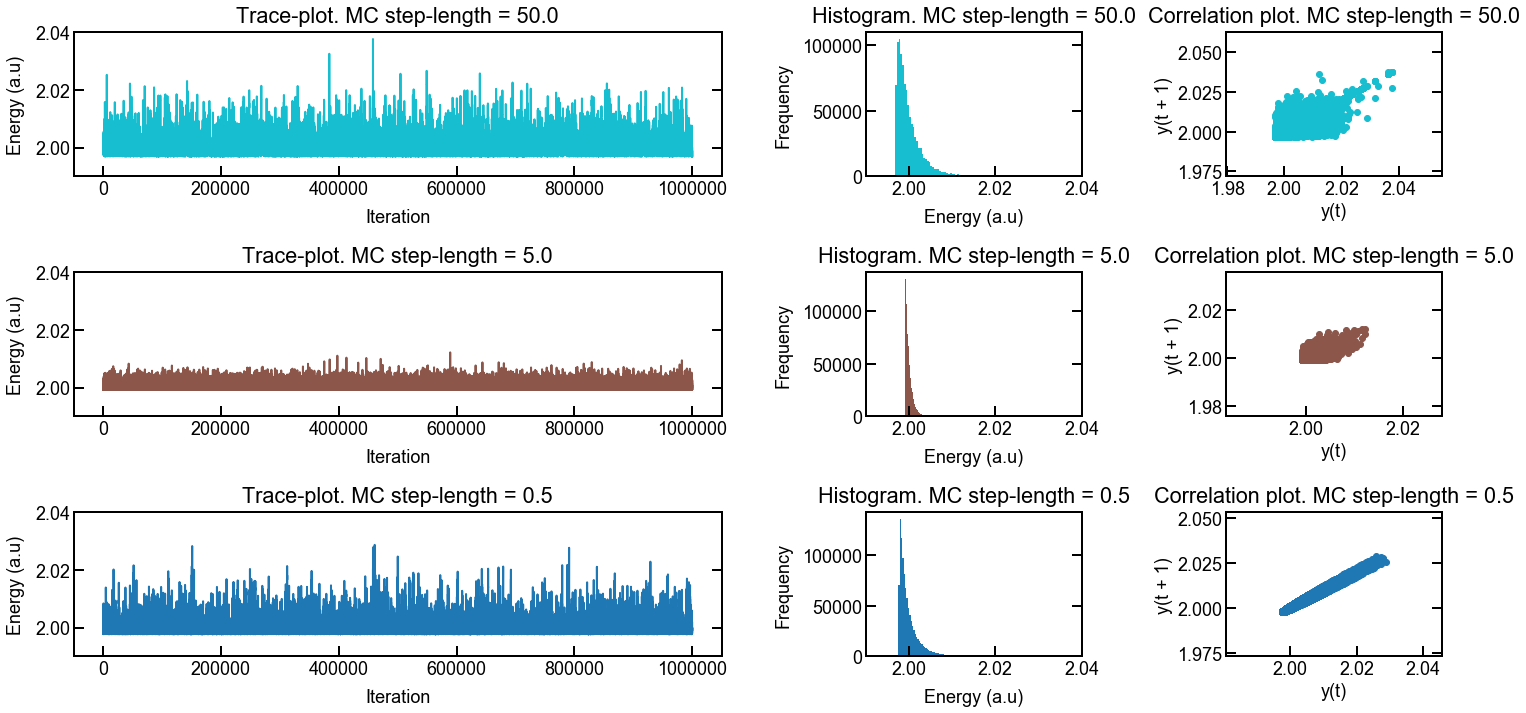
\includegraphics[width=\textwidth]{test.png}
    \caption{Various diagnostic plots for MCMC. The system is a Slater-RBM wave function for non-interacting particles with 2 particles in 2 dimensions.}
    \label{fig:rbm_mcmc_diagnostic}
\end{figure}

\begin{table}[h!]
    \centering
    \begin{tabular}{rrrr}
     MC step-length &    Energy &           Var &  Acceptance ratio \\ \hline
                0.5 &  1.999973 &  2.409328e-09 &          0.930229 \\
                5.0 &  1.999999 &  1.873899e-11 &          0.434517 \\
               50.0 &  1.999986 &  2.214887e-09 &          0.045164 \\
    \end{tabular}
    \caption{The system is a Slater-RBM wave function for non-interacting particles with 2 particles in 2 dimensions.}
    \label{tab:rbm_mcmc_diagnostic}
\end{table}
The first thing to note is the trace-plots. All methods have relatively good mixing properties, and they converge to the target distribution immediately. However, the chain for a MC step-length of 0.5 seems to have a much lower variance, and the values are more spot on. This can also be seen in table \ref{}. The variance is an order of 2 lower. When studying the chains, we are also interested in looking at the correlation between the samples. For $\detla x = 5.0$, the samples are clearly highly correlated. The reason for this is possibly that we propose new position that are to different from the last step, many proposals will then be rejected, and we will stay in the same position multiple steps. Choosing the step-length smaller seems to give less correlated. However, when choosing it to small the samples seems to be more correlated again. This can be seen from the correlation plot for $\delta x = 0.05$. 
\\
\\
We can now compare it to the results from using importance sampling instead of the brute-force sampling. 
\\
\\
In figure \ref{} and table \ref{}, the results are shown for different step sizes. 
\\
\\
For the Boltzmann machine we have som extra flexibility compared to the standard Slater and Slater-Jastrow wavefunctions. the number of nodes in the hidden layer can play an important role in the accuracy of the estimates. We will now use importance sampling with step-length = ... for the rest of the analysis, and compare the convergence for different number of hidden nodes.  
\subsubsection{Slater-NN}
As before, we will start by studying the step-length of the brute-force proposal algorithm before we look at importance sampling. The same steps as for the RBM will be conducted to test different step-lengths. 
\\
\\
The results are shown in 
\subsubsection{Brute Force Metropolis}
Looking at the trace-plots in figure \ref{}, we note that a step-length of ... seems to give good properties. For ... and ..., the chain gets stuck on certain values for a longer period of time, which restricts the chain from exploring other values. In table \ref{} the variance are shown, together with the ... 
\subsubsection{Importance Sampling Metropolis}
As for the brute-force method
\subsection{Optimization}
When the Markov Chain converges properly and produces accurate gradients and local energies, the next step is to find the optimal way to actually update the variational parameters of the model.  Again, this will depend on the system. The standard gradient descent and the adam algorithm will be compared for varying parameters.
\subsubsection{Gradient descent}
In this section the convergence of the gradient descent method is studied. In figure \ref{} the results for different learning rates are shown. 
\subsubsection{Adam}
\subsection{Energy}
Now that the optimal parameters and methods are found, they will be used to calculate the energy of a system of non-interacting particles. The analytical results is used as a benchmark for the methods.
\\
\\
For the non-interacting system, we assume to get very got results for every combination of the Wavefunction elements. The results from running 50 optimization steps with $10^5$ Monte Carlo steps in each iteration are shown in table:
\begin{table}[h!]
\centering
\begin{tabular}{c|c}
    Wavefunction & $\psi_{SD}\psi_{J}$  \\
    Test &  Test \\
\end{tabular}
\end{table}
We see that all wavefunction gives accurate results for the non-interacting case. 

\subsection{Electron density}
We can now study the electron density to see where the particles tends to be. 

\section{Interacting particles}
In this section systems of interacting particles in a quantum dot are studied. We no longer have easily obtained analytical expression, except for certain cases. We will mainly test over method against the system where the analytical solution are found. Our implementation is compared to previous work done on similar systems. The most interesting part is to see how the neural network compares to the restricted Boltzmann Machine. 
\\
\\
We now also want to combine all wavefunction elements to see if it is possible to get even closer to the exact value. It is interesting to see if the neural network are able to improve the results given by the rbm. This will be done by training each part separately. First, we find the optimal parameter with only the slater. Then we add the rbm and trains that. Then, we add the neural network and trains that separately as well. The results are shown in table \ref{} and figure \ref{}. 

\newpage
    
    \part{Conclusion} \label{part:conclusion}
    % \input{retrospect.tex}
    
    % \printbibliography
    
    \appendix
    %\input{diracformalism.tex}
    % \input{naturalunits.tex}
    % \input{derivationofrbm.tex}
    % \input{collectionofresults.tex}
    
    \newpage
    \nocite{*}
    %\printbibliography
    \printbibliography[type=article,title={Bibliography: Articles}]
    \printbibliography[type=book,title={Bibliography: Books}]
    \printbibliography[type=misc,title={Bibliography: Online}]
\end{document}
